\chapter{实验结果与分析}
本章,我们对使用点云对应聚类的方式和基于深度学习的点云配准方法来进行实验。
\section{数据集}
\subsection{仿真数据集}
如第\ref{sec:dataset}节所述,我们从 PointNet++ \cite{qi2017pointnet++} 的预采样 Modelnet40 数据集\cite{sunmodelnet40} 生成一个合成数据集。
我们将每个点云下采样到 $256$ 个点,并随机生成 $K$ 个变换(在我们的测试中最多为 $20$)来形成一个目标点云。目标点云也与其他物体和随机点混合,以更好地模拟真实世界的情况。

\begin{figure*}[ht]
        \centering
        \begin{subfigure}{0.4\textwidth}
            \centering
            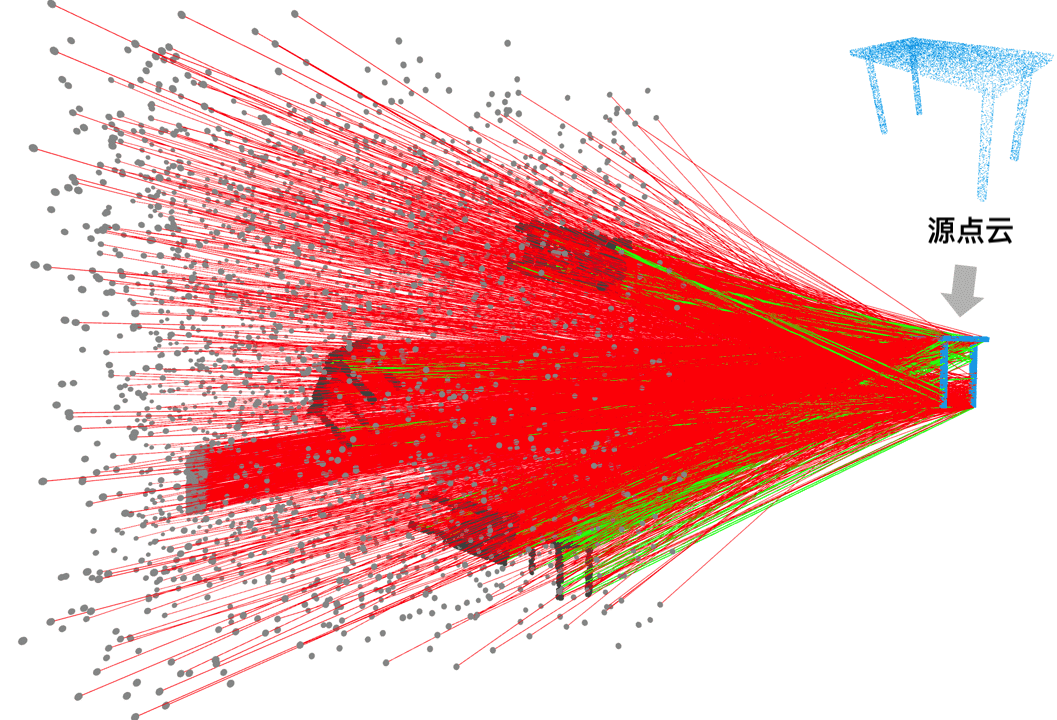
\includegraphics[height=3cm]{images/multi-input-corrs.png}
              \caption{输入匹配关系(离群点比重 : $95.5\%$) }
              \label{fig:multi-corrs}
          \end{subfigure}
          \begin{subfigure}{0.45\textwidth}
            \centering
            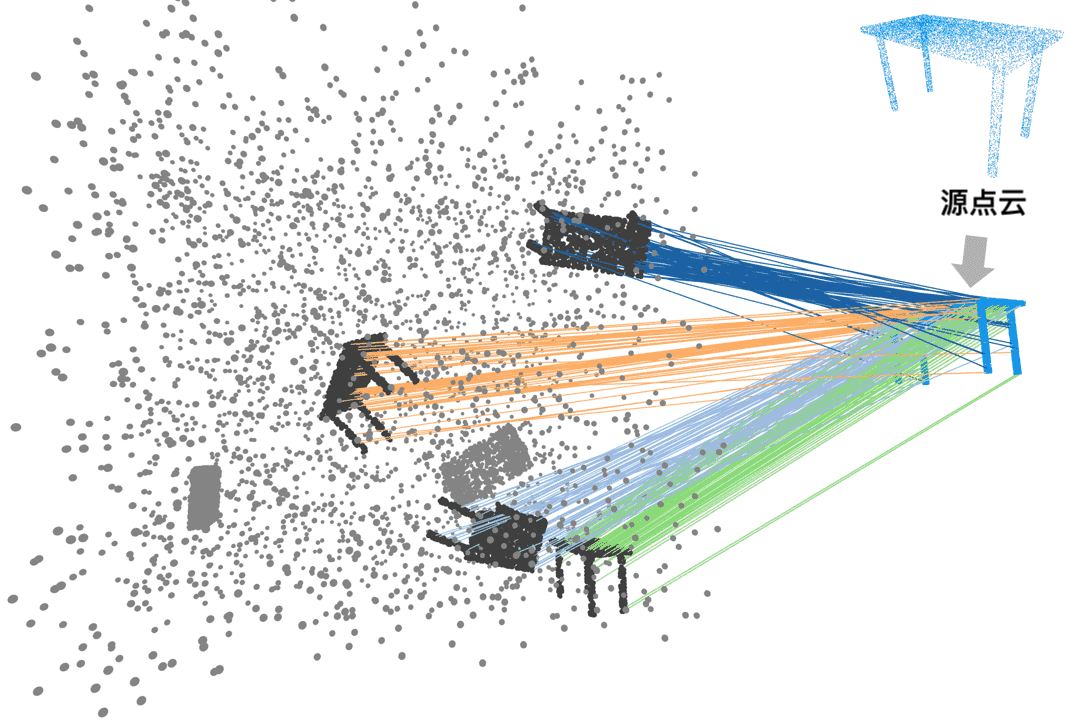
\includegraphics[height=3cm]{images/multi-cluster-corrs.png}
              \caption{我们的聚类结果}
              \label{fig:multi-cluster-corrs}
          \end{subfigure}
      
      
          \begin{subfigure}{0.18\textwidth}
            \centering
            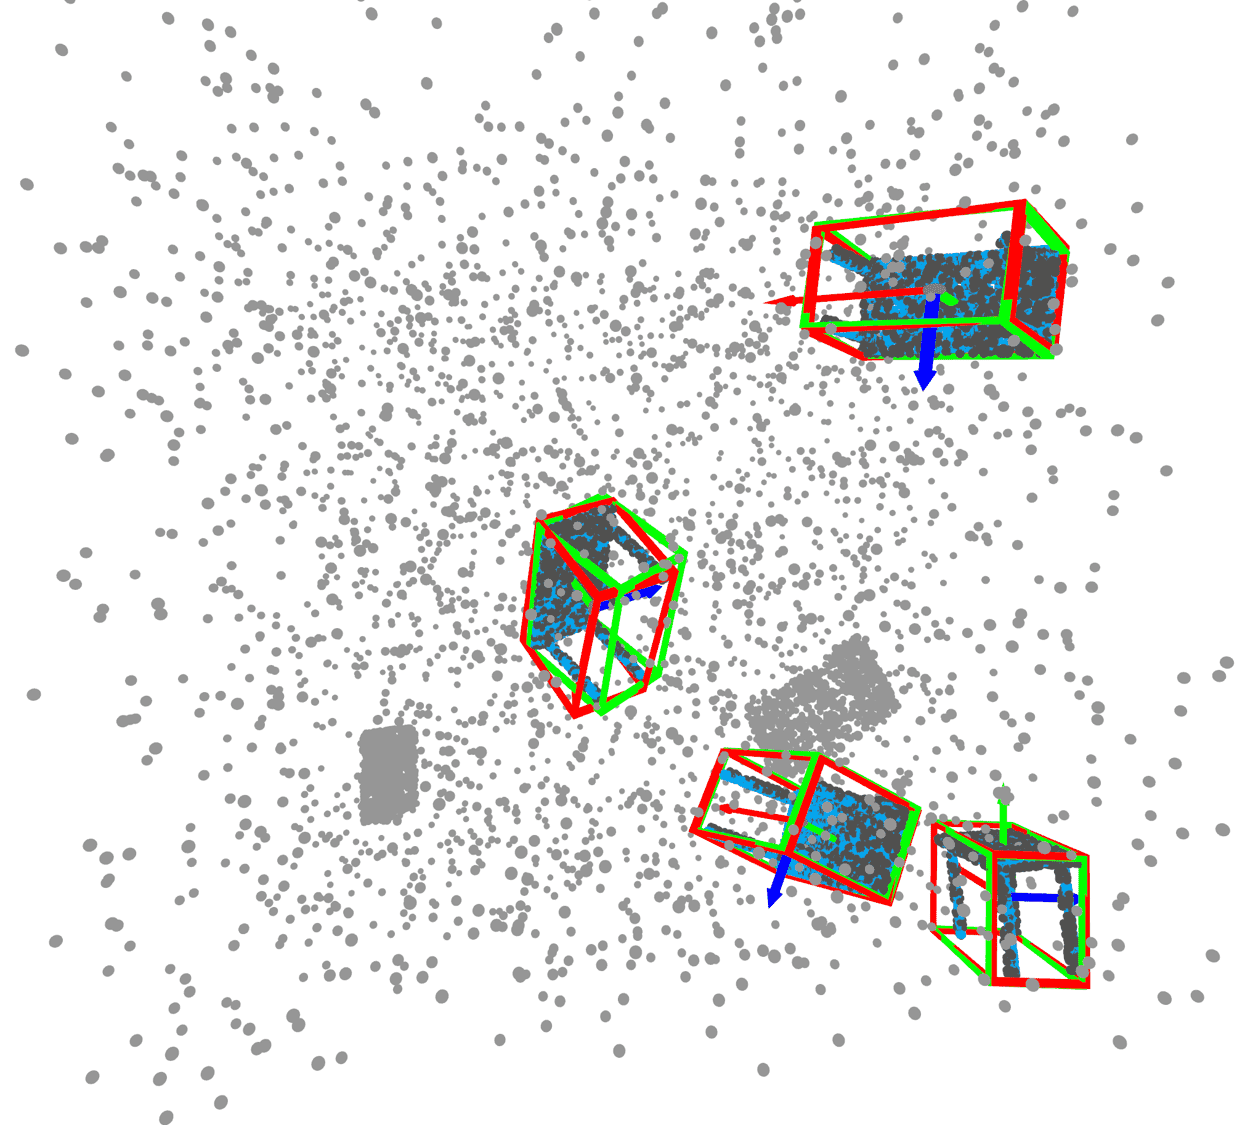
\includegraphics[height=2.8cm]{images/multi-ours.png}
              \caption{Ours}
              \label{fig:multi-result}
          \end{subfigure}
          \begin{subfigure}{0.18\textwidth}
            \centering
            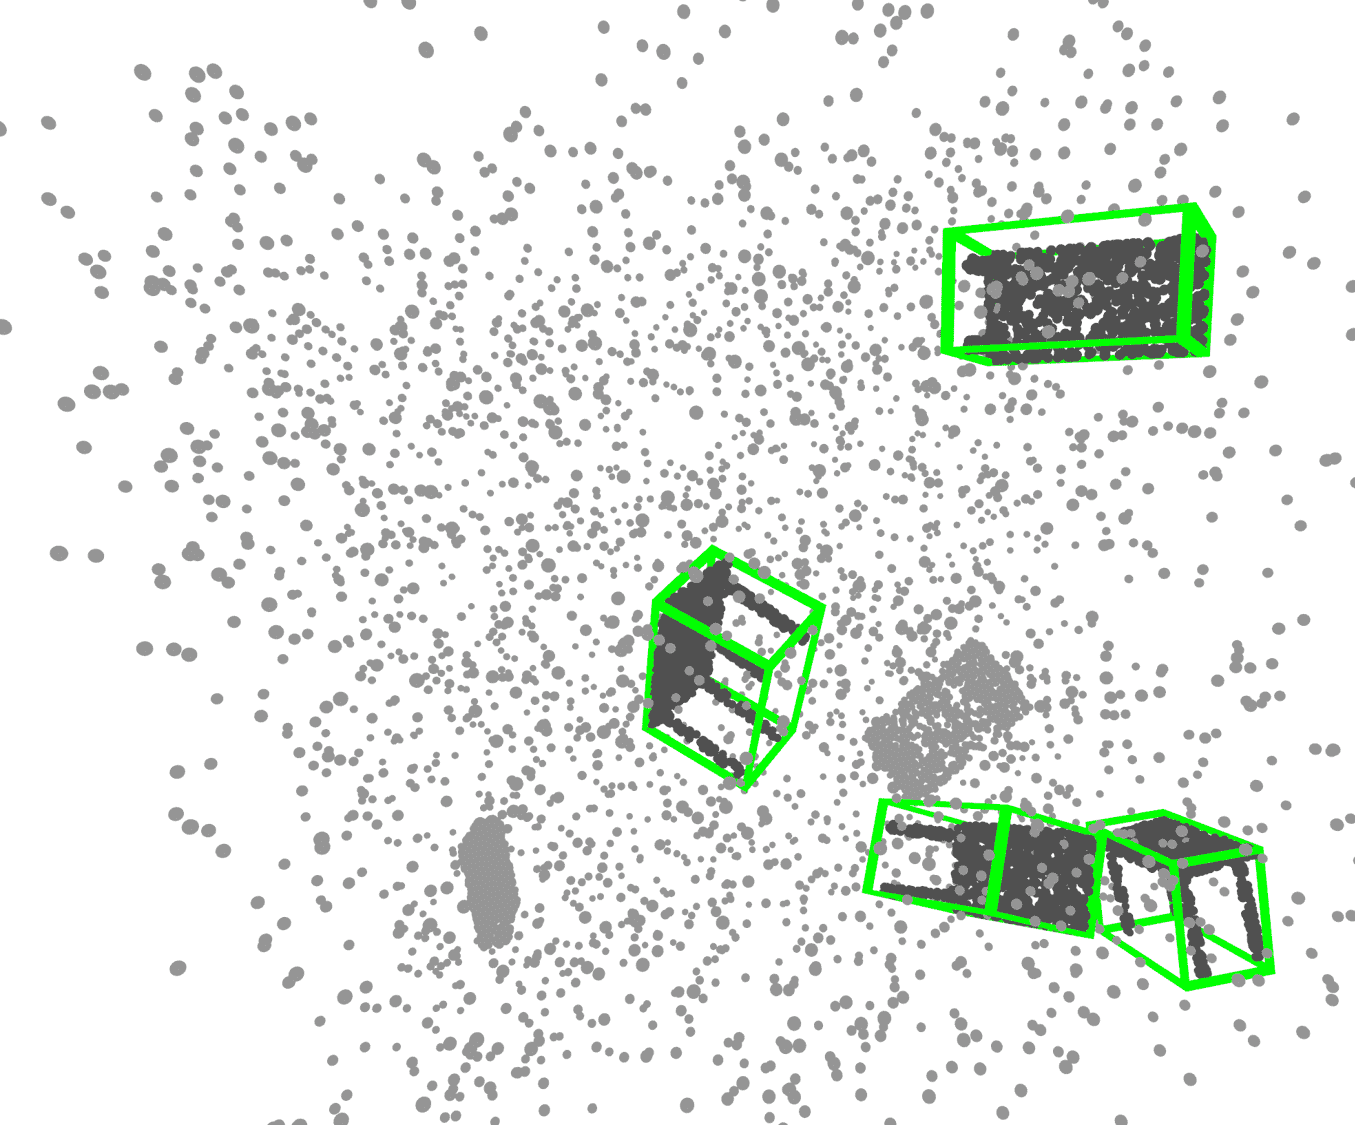
\includegraphics[height=2.8cm]{images/multi-tlinkage.png}
              \caption{T-Linkage\cite{magri2014t}}
              \label{fig:multi-tlinkage1}
          \end{subfigure}
          \begin{subfigure}{0.2\textwidth}
            \centering
            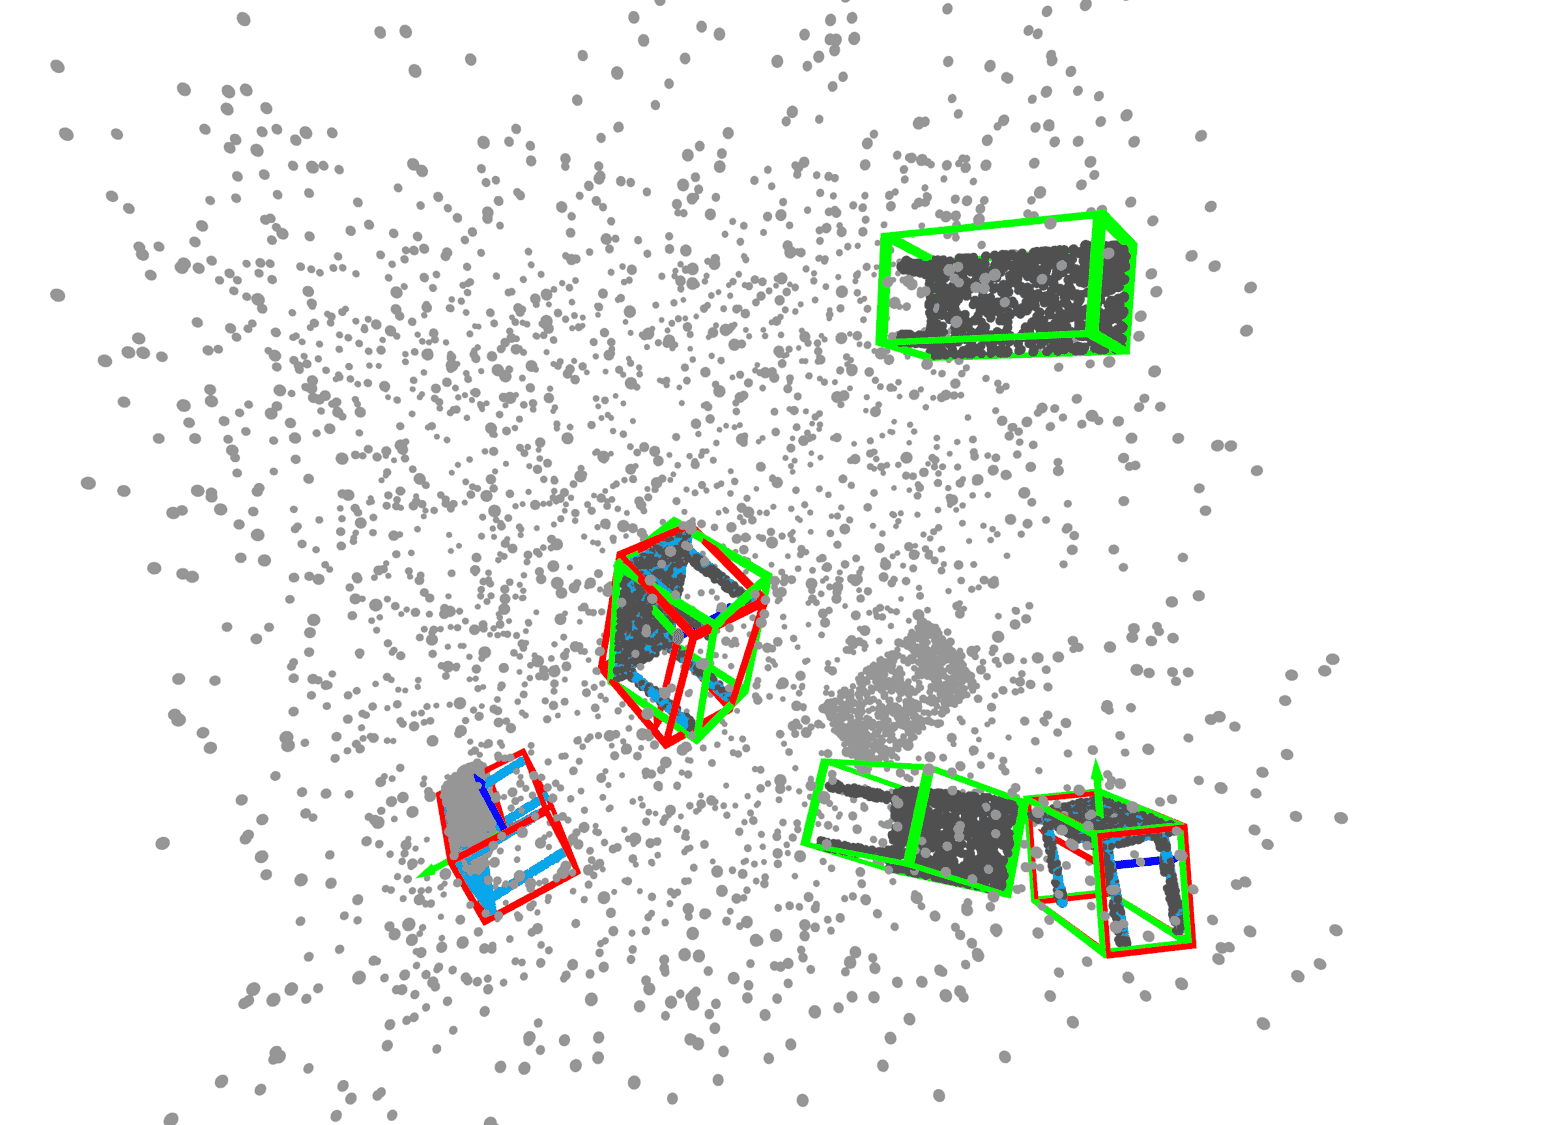
\includegraphics[height=2.8cm]{images/multi-progx.png}
              \caption{Progressive-X\cite{zhao2021progressive}}
              \label{fig:multi-prox}
          \end{subfigure}
          \begin{subfigure}{0.2\textwidth}
            \centering
            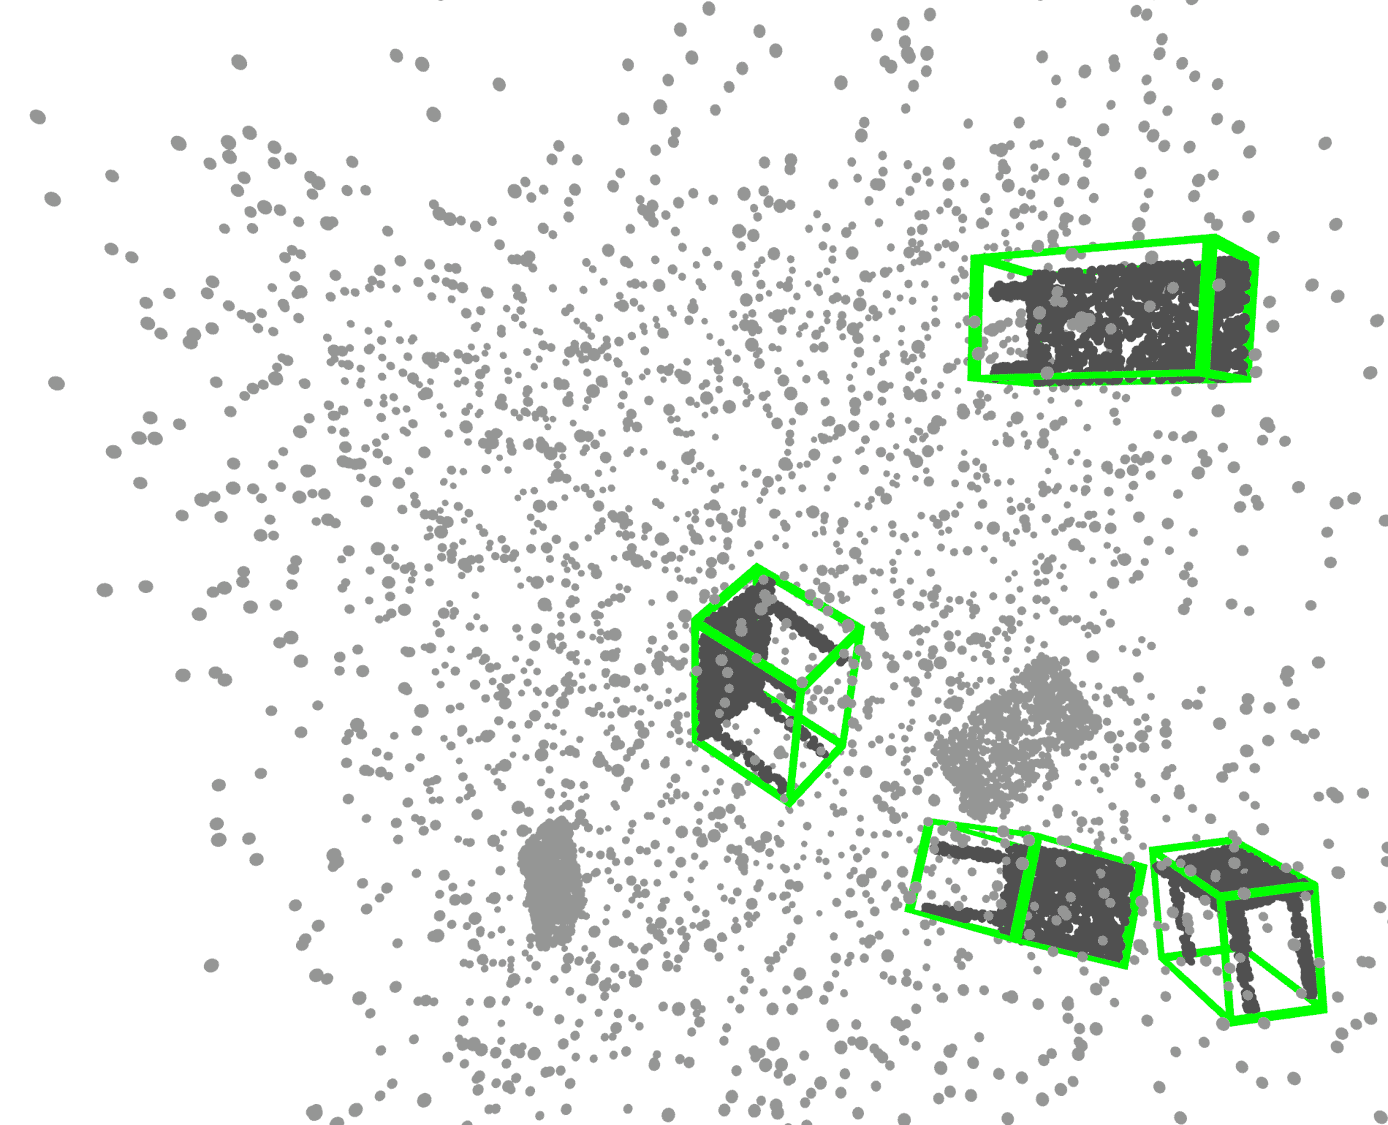
\includegraphics[height=2.8cm]{images/multi-consac.png}
              \caption{CONSAC\cite{kluger2020consac}}
              \label{fig:multi-consac}
          \end{subfigure}
          \begin{subfigure}{0.18\textwidth}
            \centering
            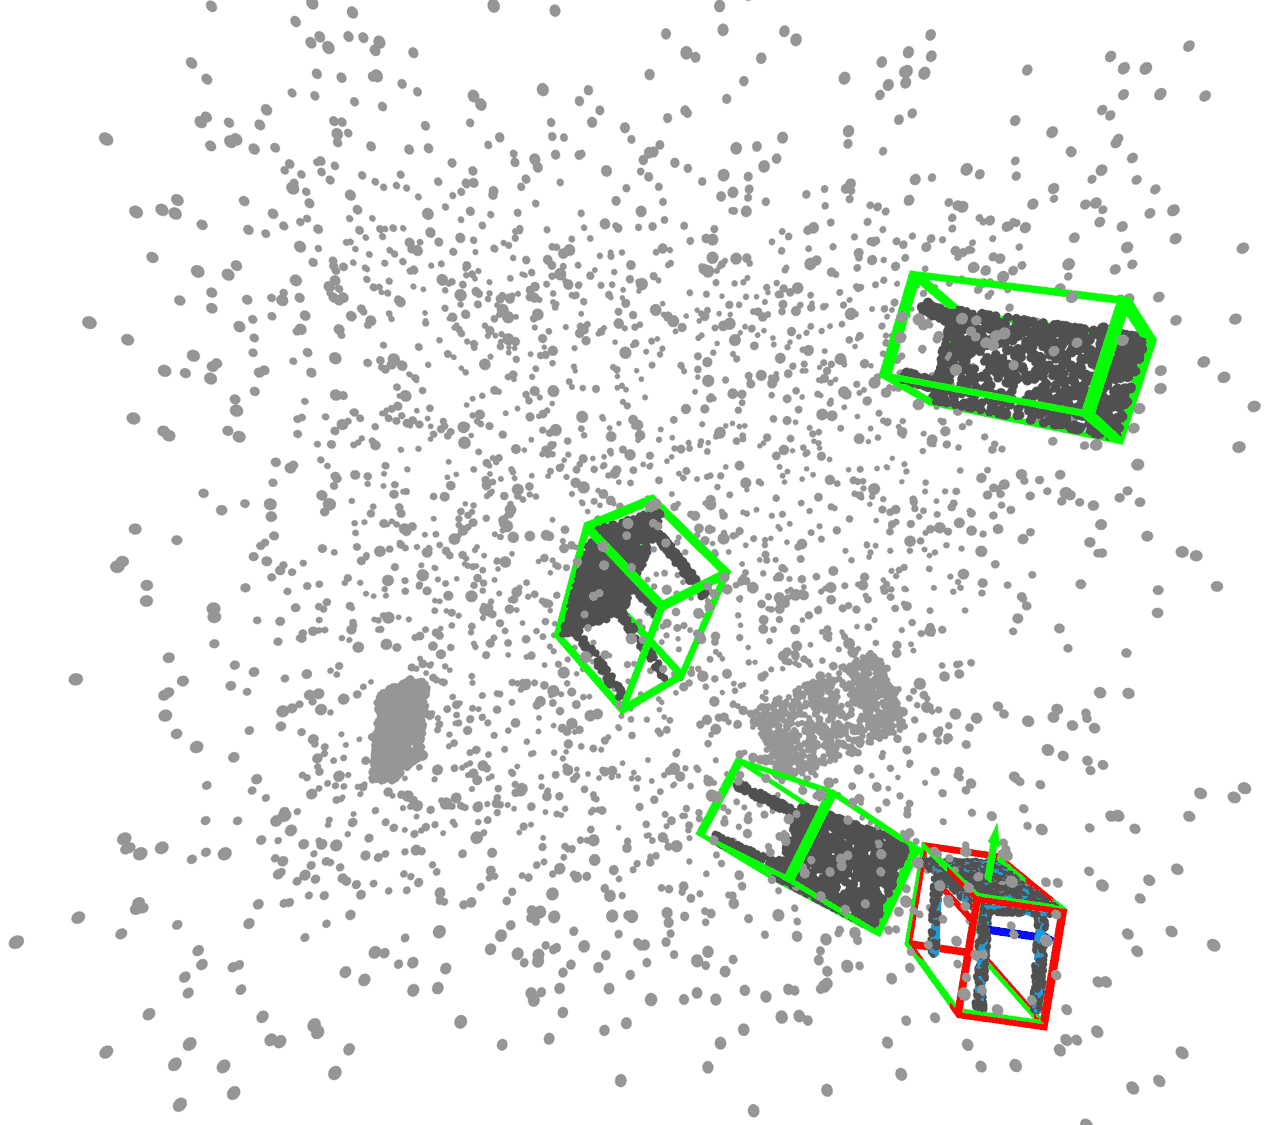
\includegraphics[height=2.8cm]{images/multi-teaser.png}
              \caption{TEASER\cite{yang2020teaser}}
              \label{fig:multi-teaser}
          \end{subfigure}
          % \begin{subfigure}{0.18\textwidth}
          %   \centering
          %   \includegraphics[height=2.5cm]{scan2cad-cad-ransac1.png}
          %     \caption{RANSAC}
          %     \label{fig:scan2cad_cad-ransac1}
          % \end{subfigure}
      
      %\includegraphics[width=0.9\columnwidth]{figure/} % Reduce the figure size so that it is slightly narrower than the column. Don't use precise values for figure width.This setup will avoid overfull boxes.
      \caption{\textbf{在仿真数据集上的结果。} (a) 通过匹配 PREDATOR\cite{huang2021predator} 特征得到的输入对应关系。内点和离群点分别用绿色和红色显示。 (b) 我们的聚类结果用不同的颜色显示(只显示内点)。在 (c-g) 中,我们用红色框显示估计的位姿,用绿色框显示真实位姿。我们的方法 (c) 配准了所有实例。T-linkage (d) 和 CONSAC (f) 无法配准任何实例。Progressive-X (e) 配准了 2 个实例,但产生了错误的配准。TEASER (g) 配准了一个实例。}
      \label{fig:predatormm}
\end{figure*}

\subsection{真实数据集}
Scan2CAD\cite{avetisyan2019scan2cad} 是一个数据集,它将 ShapeNet\cite{chang2015shapenet} CAD 模型与 ScanNet\cite{dai2017scannet} 点云中的对象实例对齐。部分扫描有多个已对齐的 CAD 模型和标注的姿态。我们选择那些包含多个 CAD 模型的扫描作为目标点云,并从 CAD 模型中采样源点云进行测试。我们为配准测试生成了 173 个样本,其中大多数样本包含 $2 \sim 5$ 个实例。
请注意,在每个点云中,Scan2CAD 中仅标注了部分实例。这意味着我们无法使用部分标注的姿态正确评估性能,如准确率和召回率。为解决这个问题,我们仅在目标点云中标注的物体的真实边界框内匹配点以生成对应关系。同样,我们使用 PREDATOR\cite{huang2021predator} 和 D3Feat\cite{bai2020d3feat} 进行点匹配,两者都是使用 Scan2CAD 数据集中的 1028 个训练样本和 187 个验证样本进行微调的。

\begin{figure*}[ht]
        \centering
        \begin{subfigure}{0.41\textwidth}
            \centering
            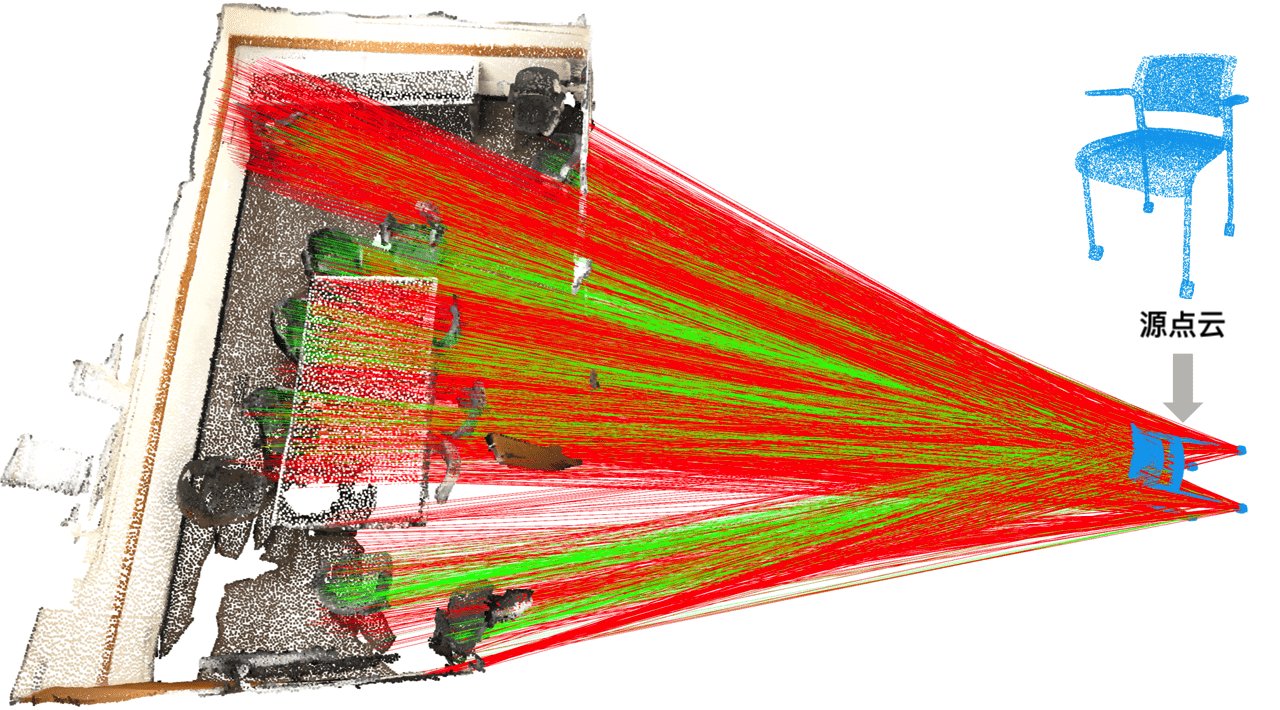
\includegraphics[height=2.8cm]{images/scan2cad-cad-input-corrs.png}
              \caption{Input correspondences}
              \label{fig:scan2cad_cad-input-corrs}
          \end{subfigure}
          \begin{subfigure}{0.41\textwidth}
            \centering
            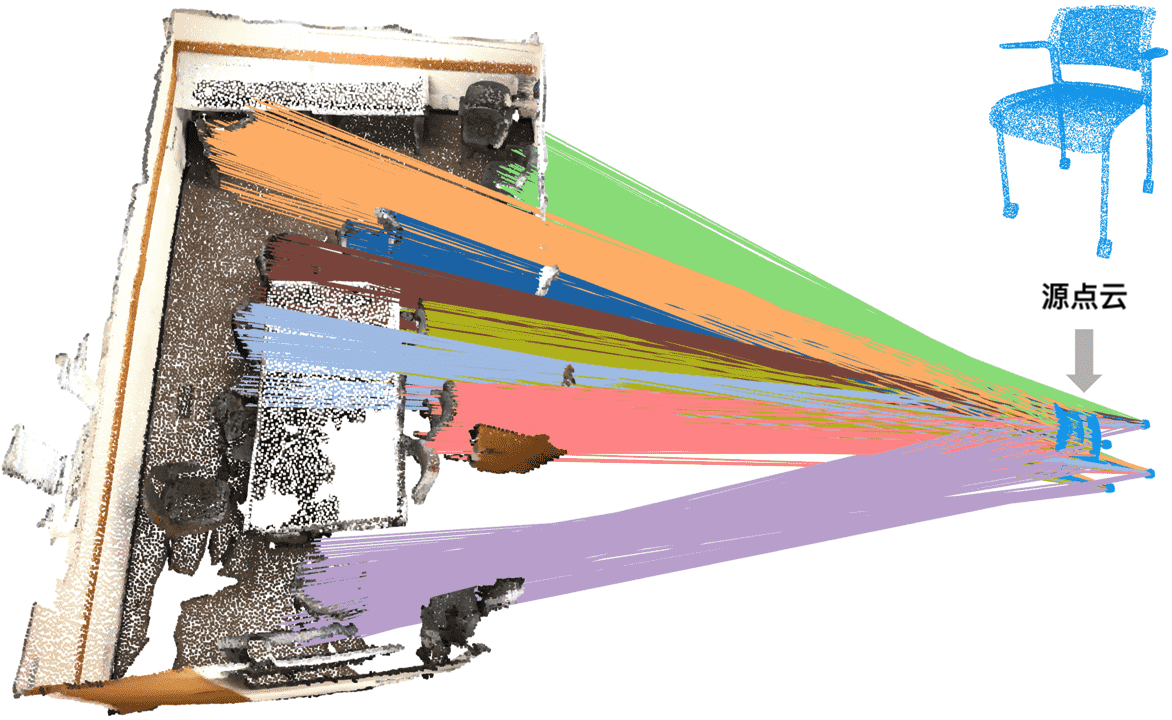
\includegraphics[height=2.8cm]{images/scan2cad-cad-cluster-corrs.png}
              \caption{Our clustering result}
              \label{fig:scan2cad_cad-cluster-corrs}
          \end{subfigure}
    
          
          \begin{subfigure}{0.18\textwidth}
            \centering
            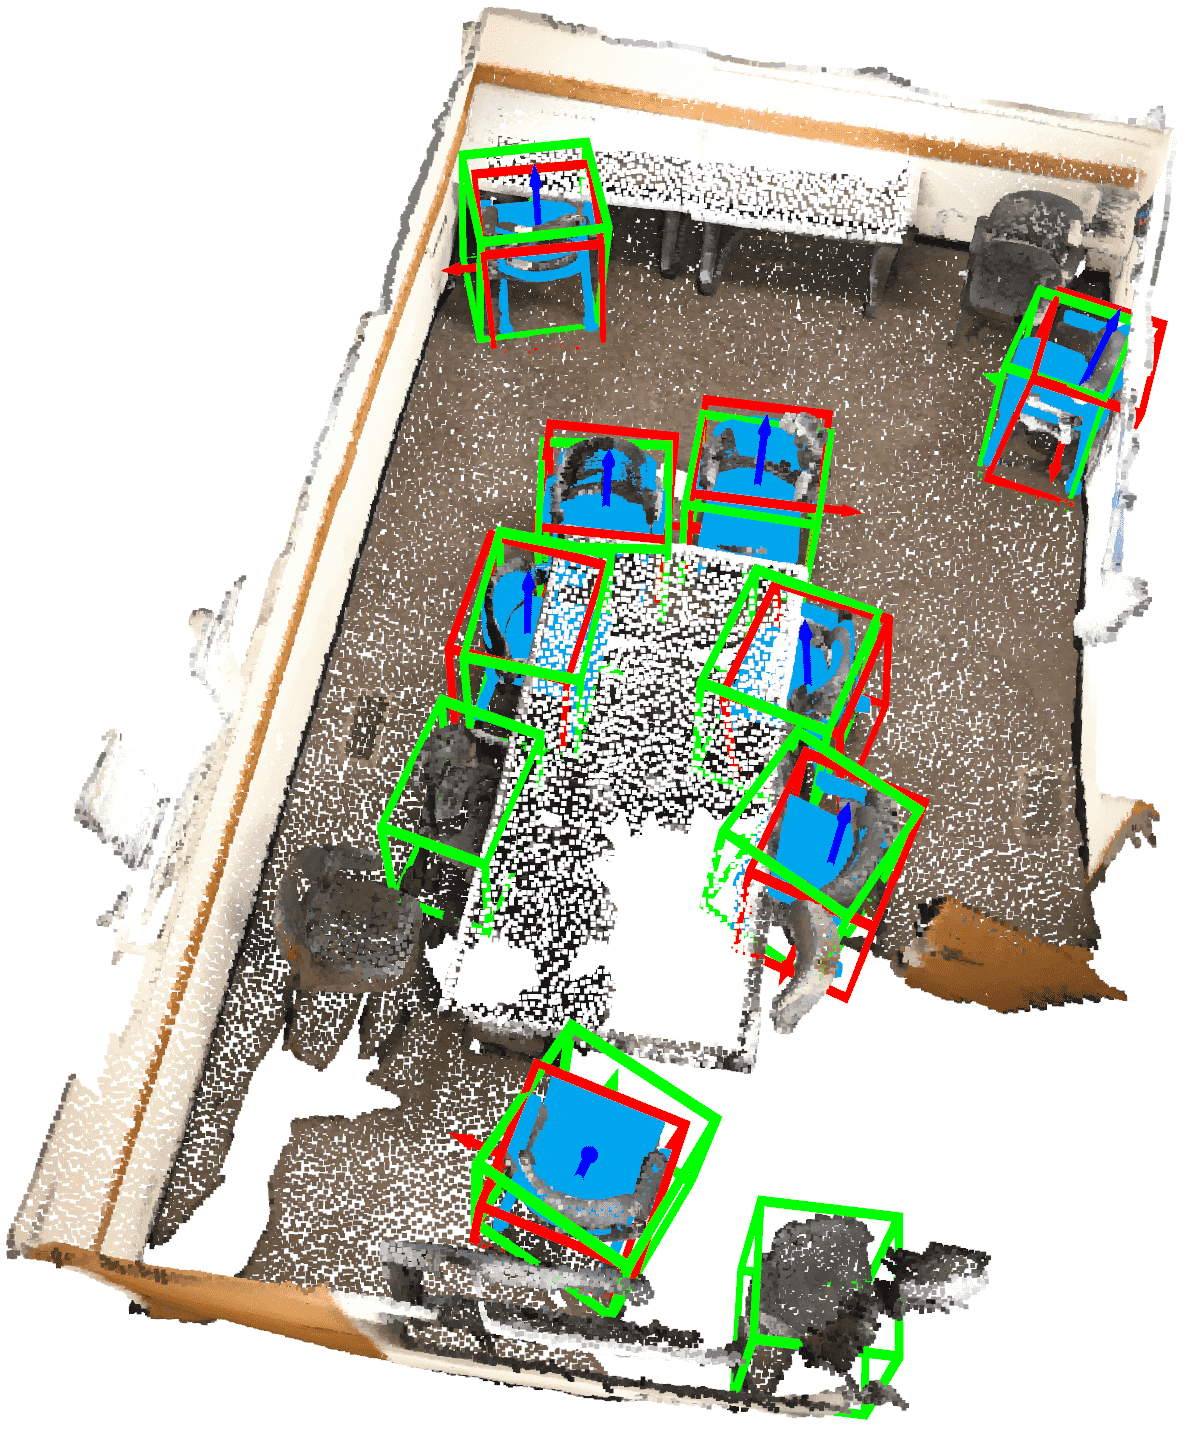
\includegraphics[height=3.3cm]{images/scan2cad-cad-ours.png}
              \caption{Ours}
              \label{fig:scan2cad_cad-result}
          \end{subfigure}
          \begin{subfigure}{0.18\textwidth}
            \centering
            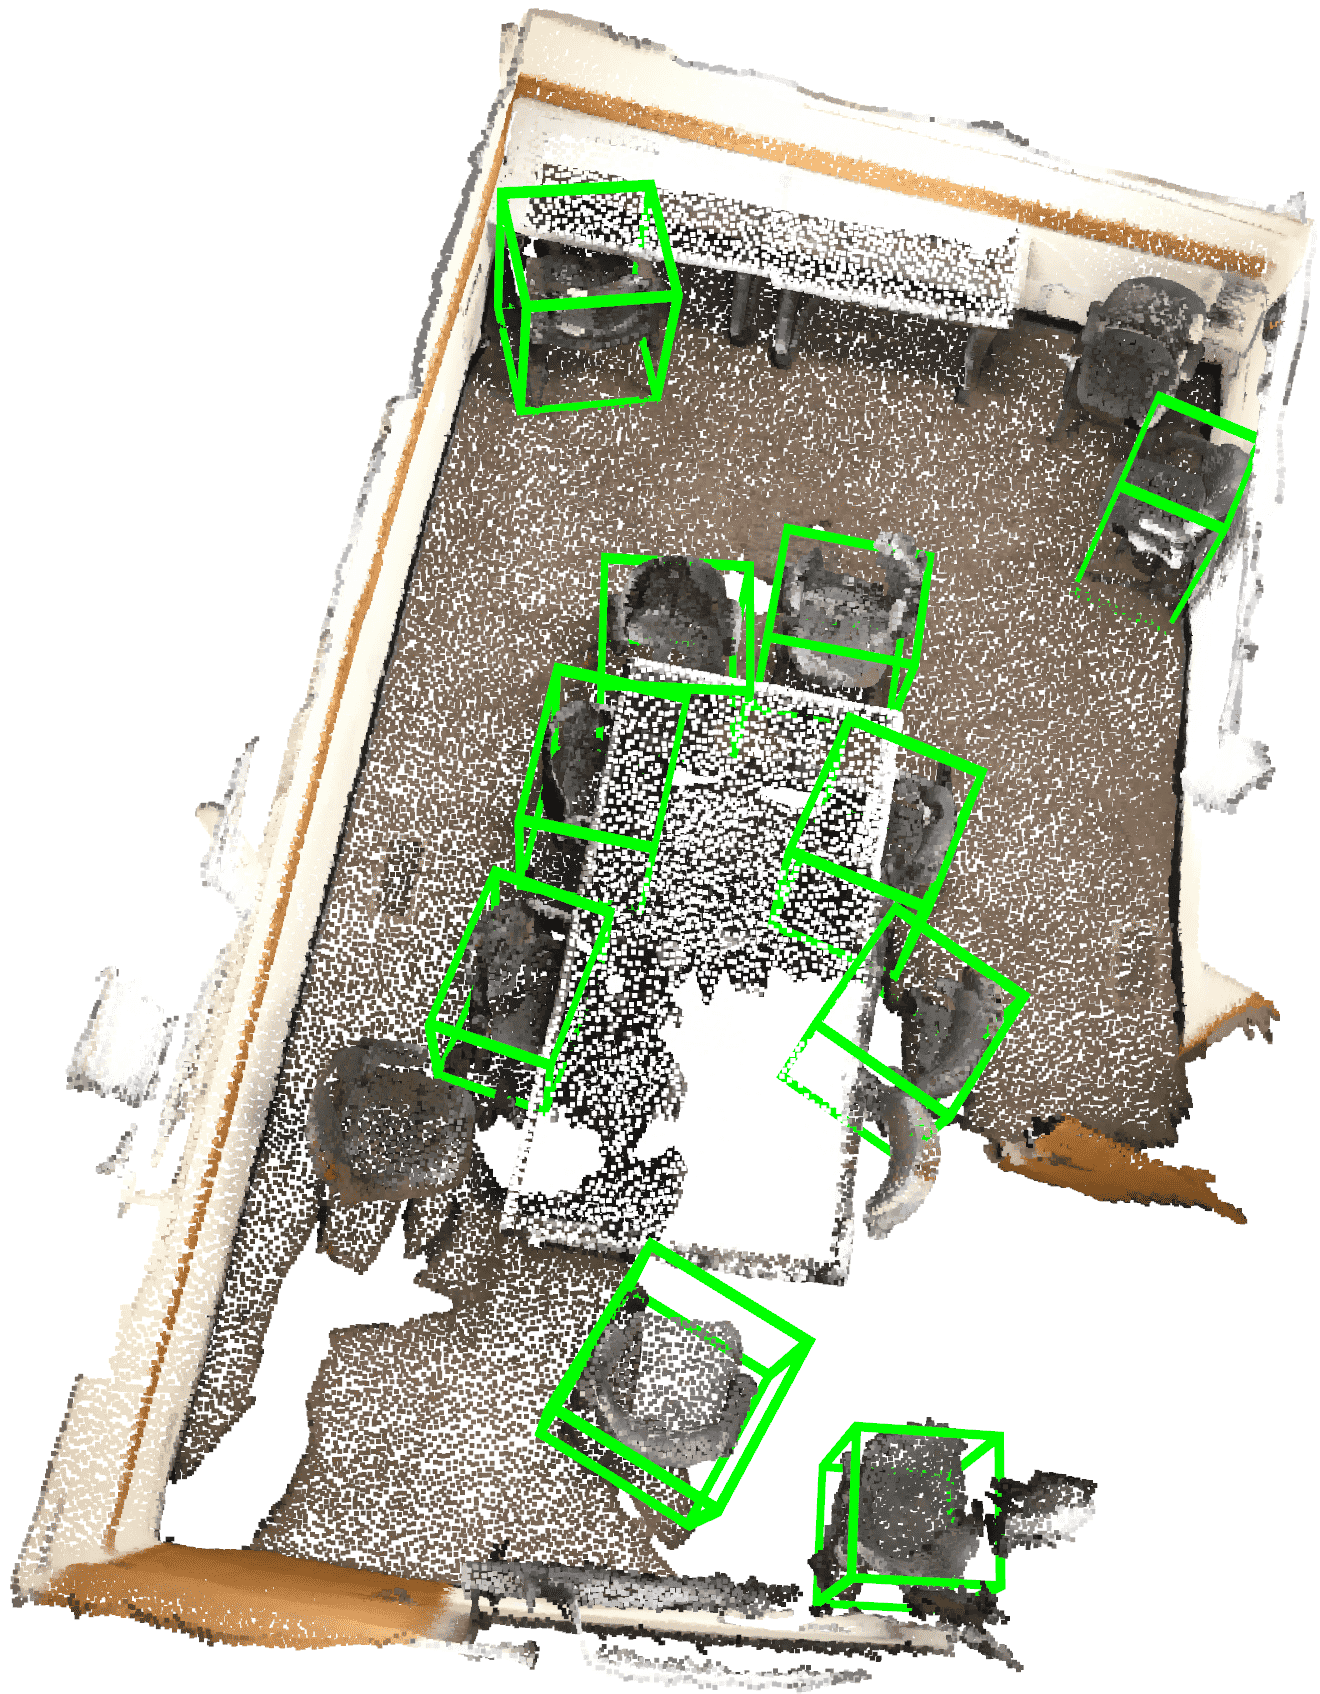
\includegraphics[height=3.3cm]{images/scan2cad-cad-tlinkage.png}
              \caption{T-linkage\cite{magri2014t}}
              \label{fig:scan2cad_cad-tlinkage}
          \end{subfigure}
          \begin{subfigure}{0.19\textwidth}
            \centering
            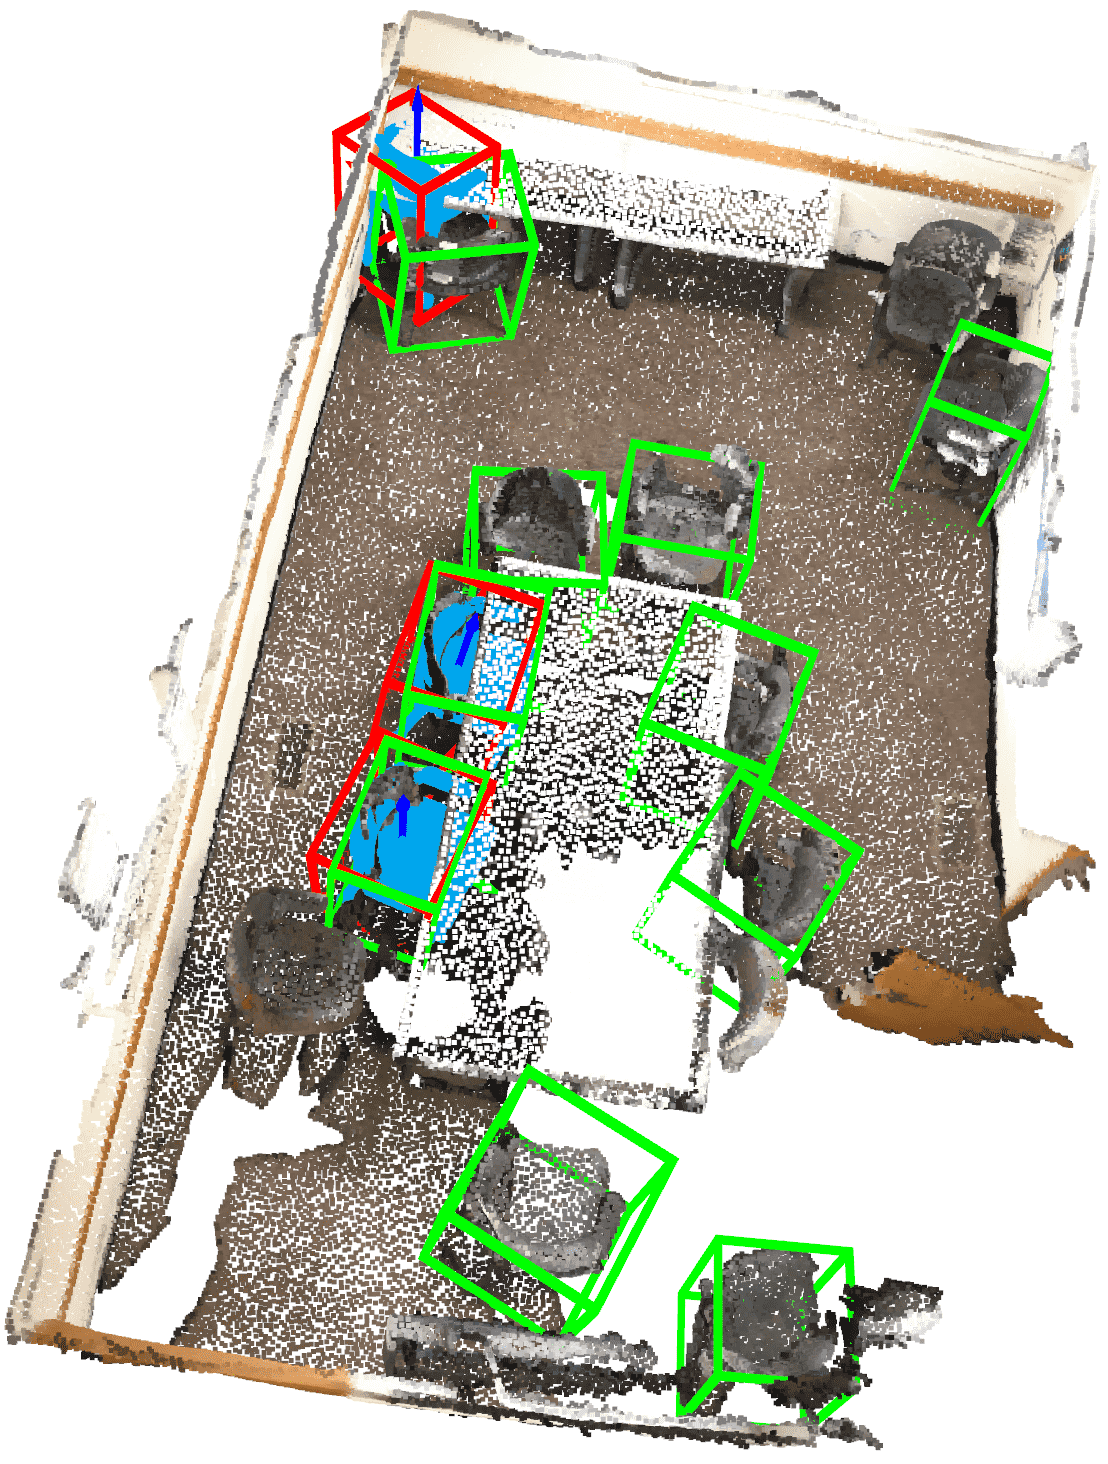
\includegraphics[height=3.3cm]{images/scan2cad-cad-progx.png}
              \caption{Progressive-X\cite{zhao2021progressive}}
              \label{fig:scan2cad_cad-prox}
          \end{subfigure}
          \begin{subfigure}{0.17\textwidth}
            \centering
            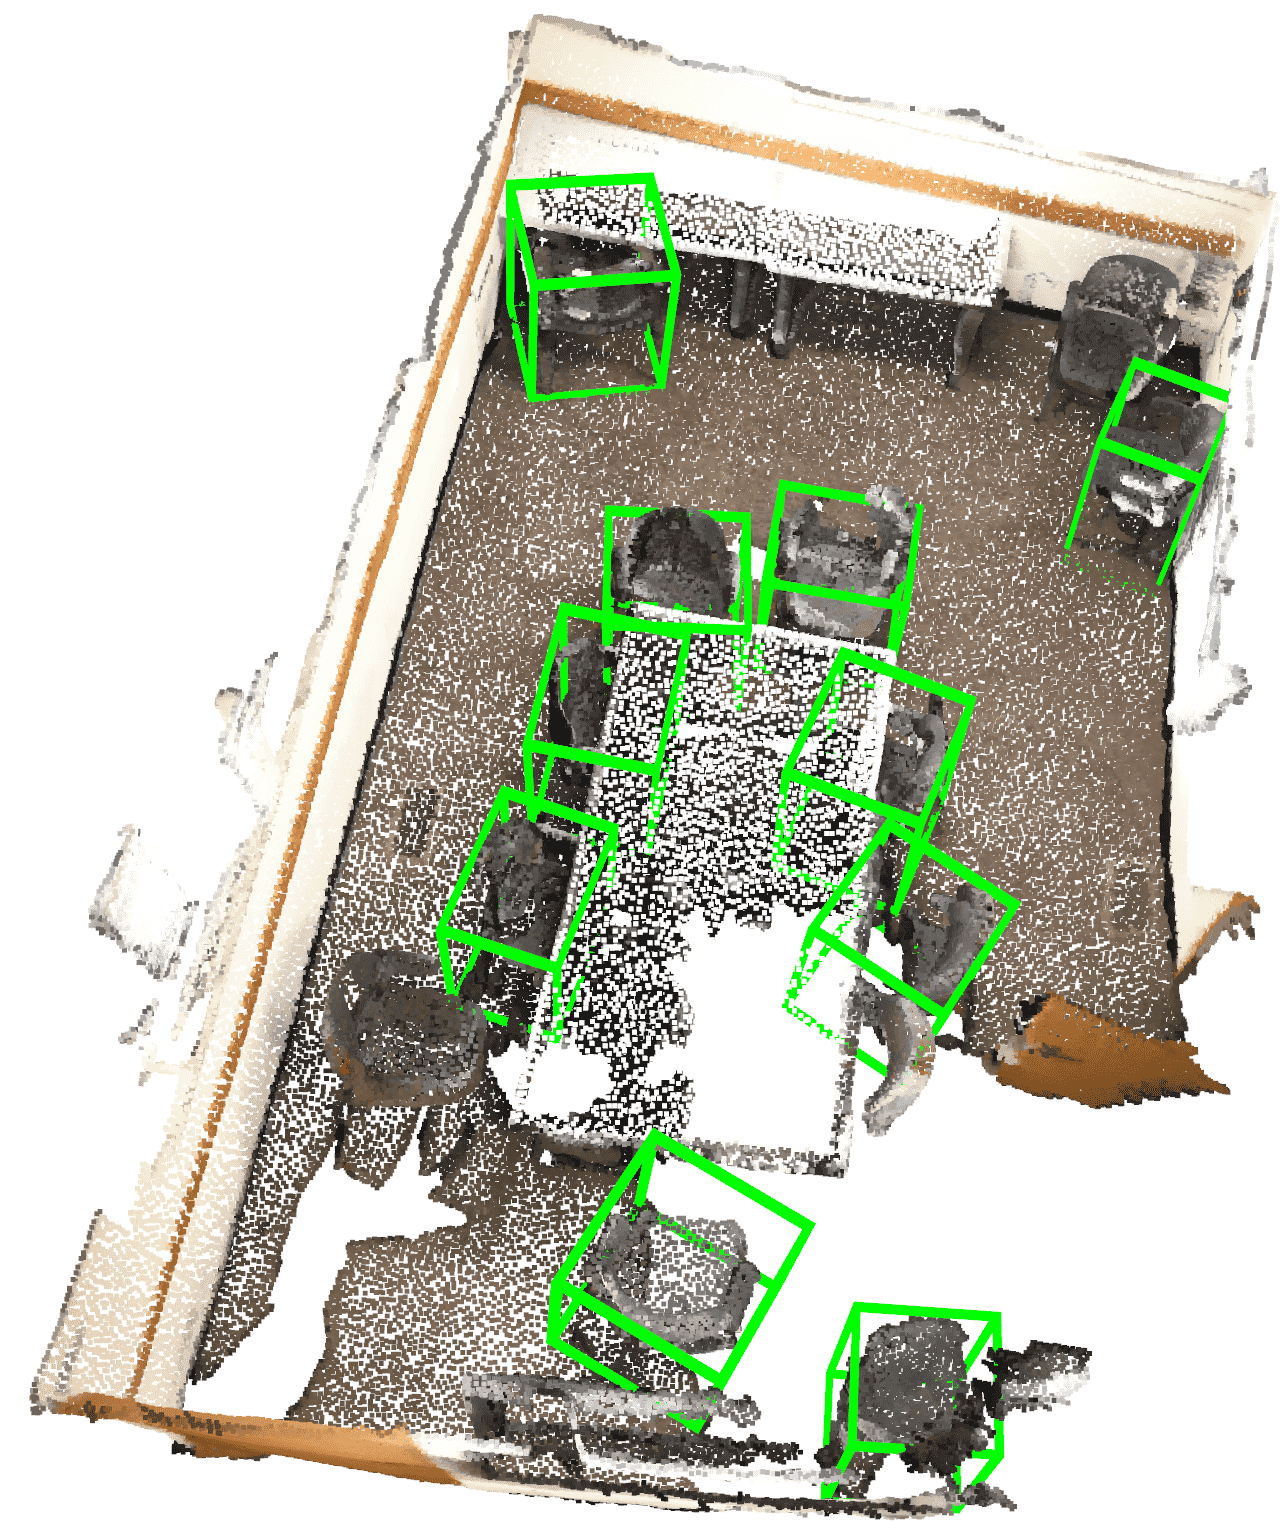
\includegraphics[height=3.3cm]{images/scan2cad-cad-consac.png}
              \caption{CONSAC\cite{kluger2020consac}}
              \label{fig:scan2cad_cad-consac}
          \end{subfigure}
          \begin{subfigure}{0.18\textwidth}
            \centering
            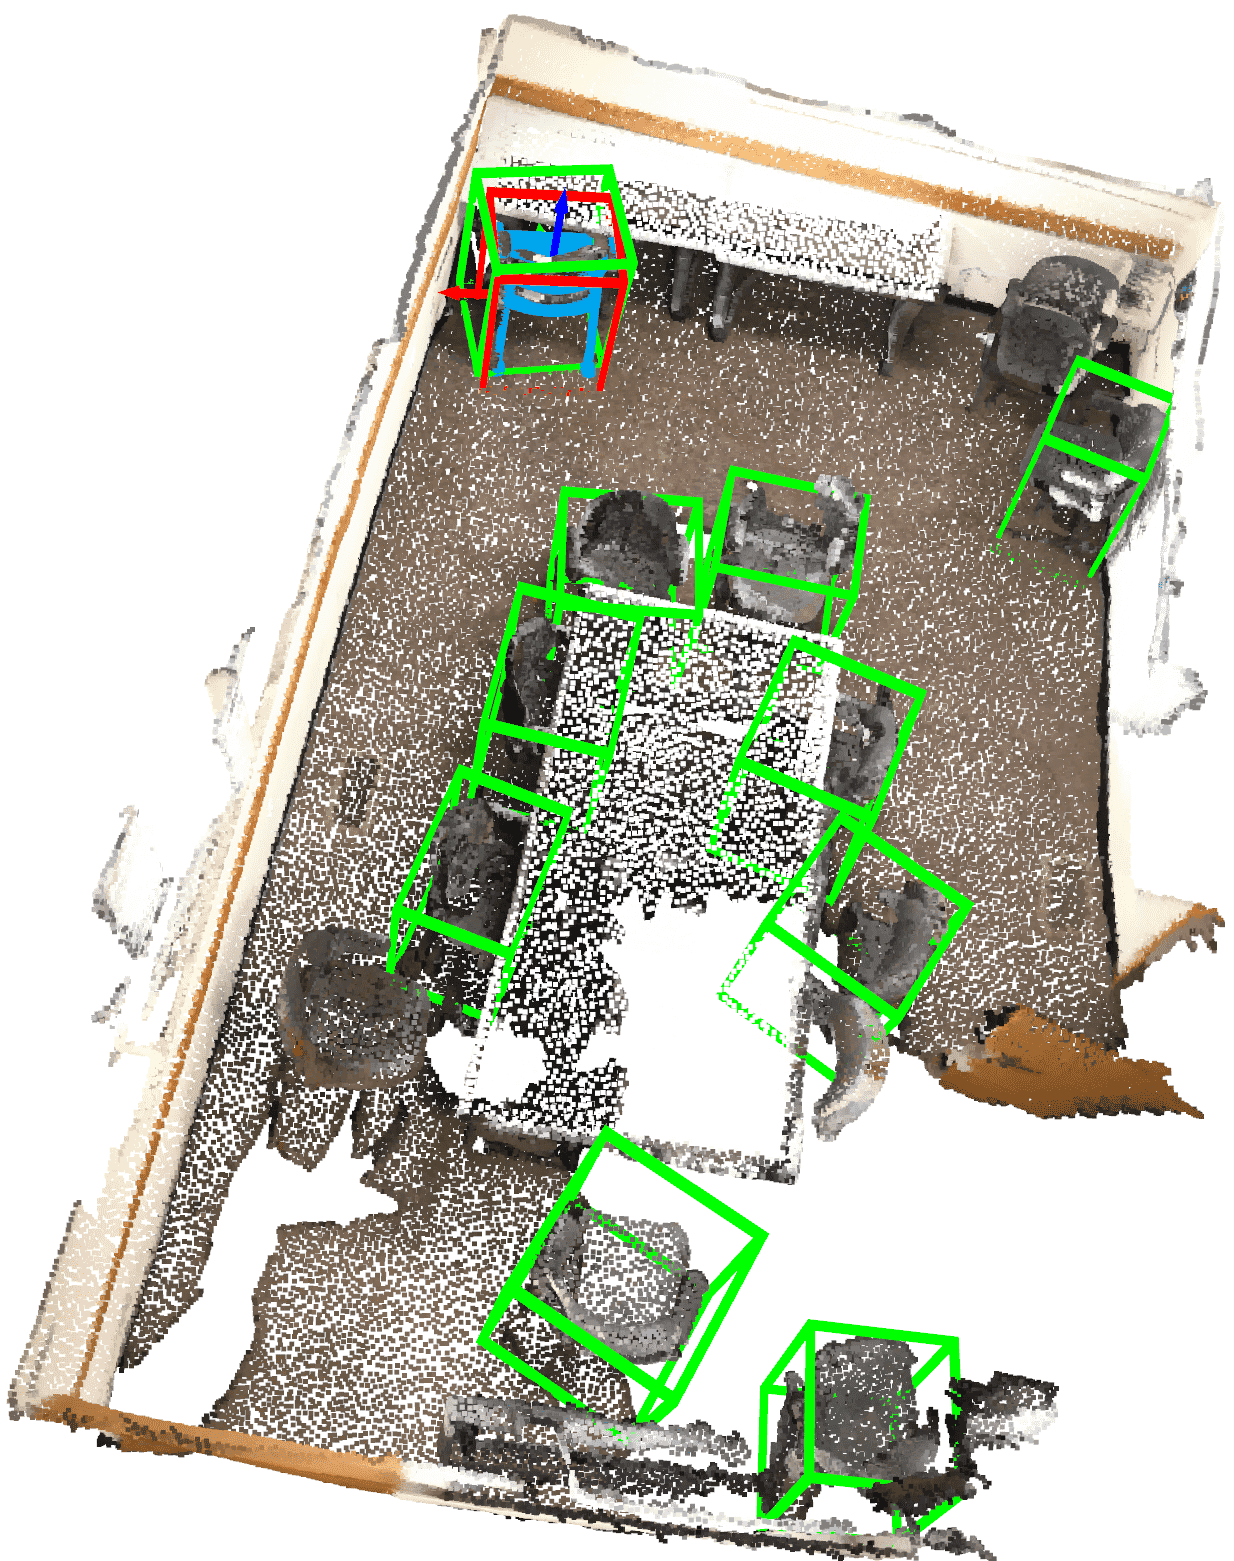
\includegraphics[height=3.3cm]{images/scan2cad-cad-teaser.png}
              \caption{TEASER\cite{yang2020teaser}}
              \label{fig:scan2cad_cad-teaser}
          \end{subfigure}
          % \begin{subfigure}{0.15\textwidth}
          %   \centering
          %   \includegraphics[height=3cm]{scan2cad-cad-ransac.png}
          %     \caption{RANSAC}
          %     \label{fig:scan2cad_cad-ransac}
          % \end{subfigure}
          \caption{\textbf{Scan2CAD 结果。} (a) 通过匹配 PREDATOR \cite{huang2021predator} 特征得到的输入对应关系。内点和离群点分别用绿色和红色显示。 (b) 我们的聚类结果用不同颜色显示(仅显示内点)。在 (c-g) 中,我们将估计的姿态用红色框显示,将真实姿态用绿色框显示。我们的方法 (c) 正确地对齐了 8 个实例。T-Linkage (d) 和 CONSAC (f) 未能配准任何实例。Progressive-X (e) 配准了 3 个实例。TEASER (g) 配准了一个实例。}
    \label{fig:Scan2CAD-cadresult}
    \end{figure*}
    
    \begin{figure*}[ht]
        \centering
        \begin{subfigure}{0.4\textwidth}
            \centering
            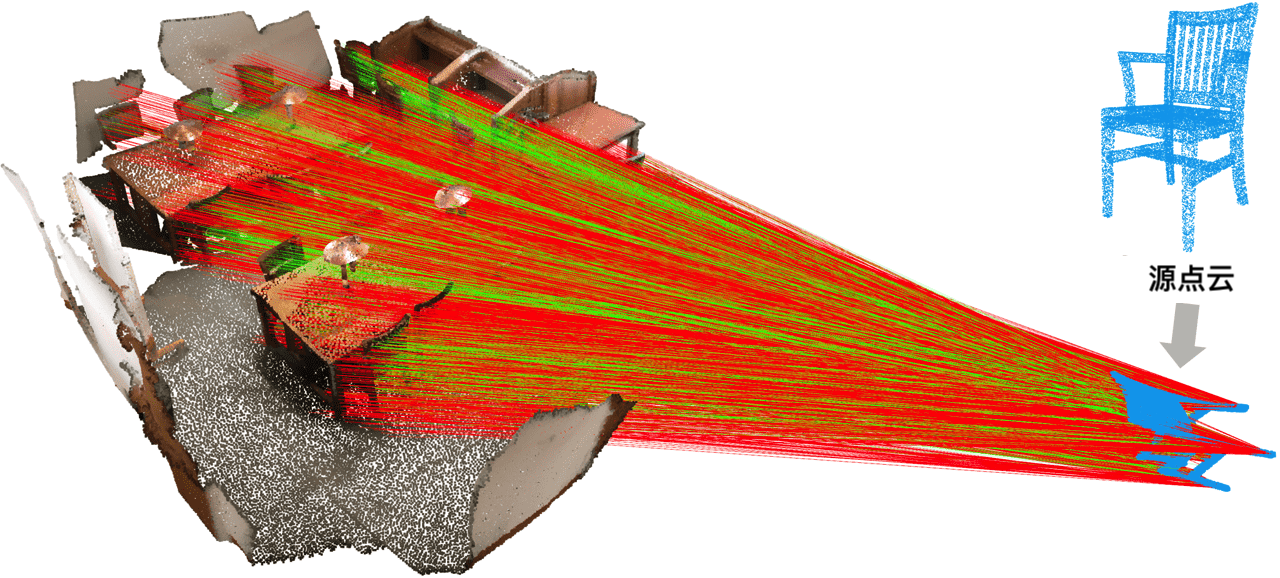
\includegraphics[height=2.8cm]{images/scan2cad-cad-input-corrs1.png}
              \caption{Input correspondences}
              \label{fig:scan2cad_cad-input-corrs1}
          \end{subfigure}
          \begin{subfigure}{0.45\textwidth}
            \centering
            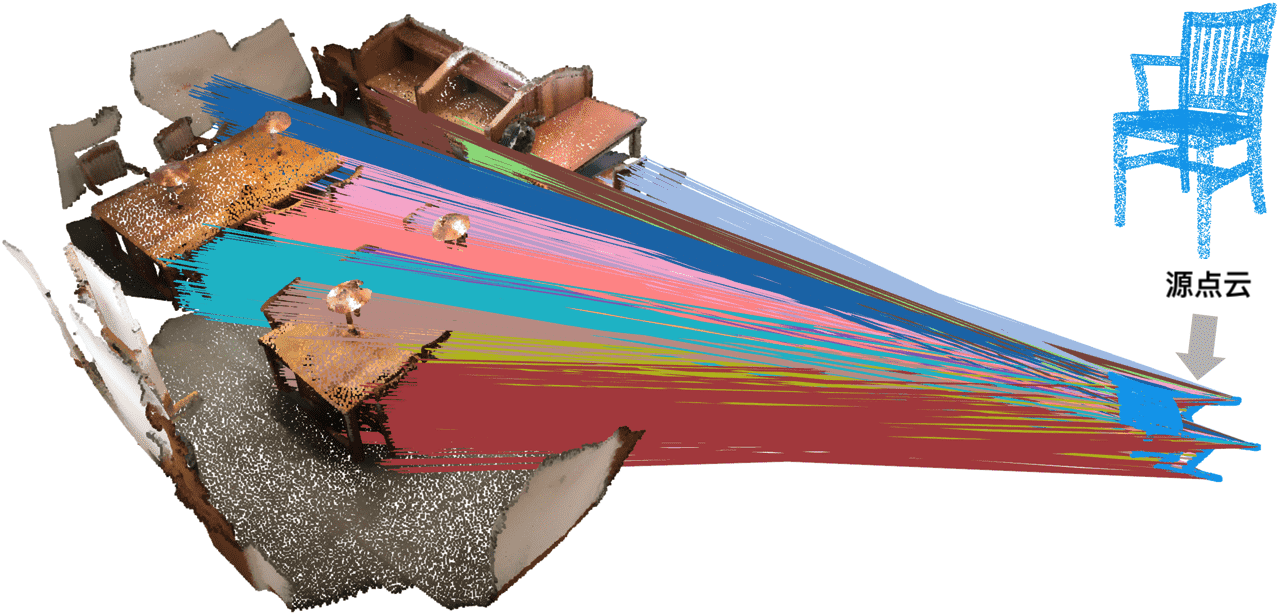
\includegraphics[height=2.8cm]{images/scan2cad-cad-cluster-corrs1.png}
              \caption{Our clustering result}
              \label{fig:scan2cad_cad-cluster-corrs1}
          \end{subfigure}
    
    
          \begin{subfigure}{0.18\textwidth}
            \centering
            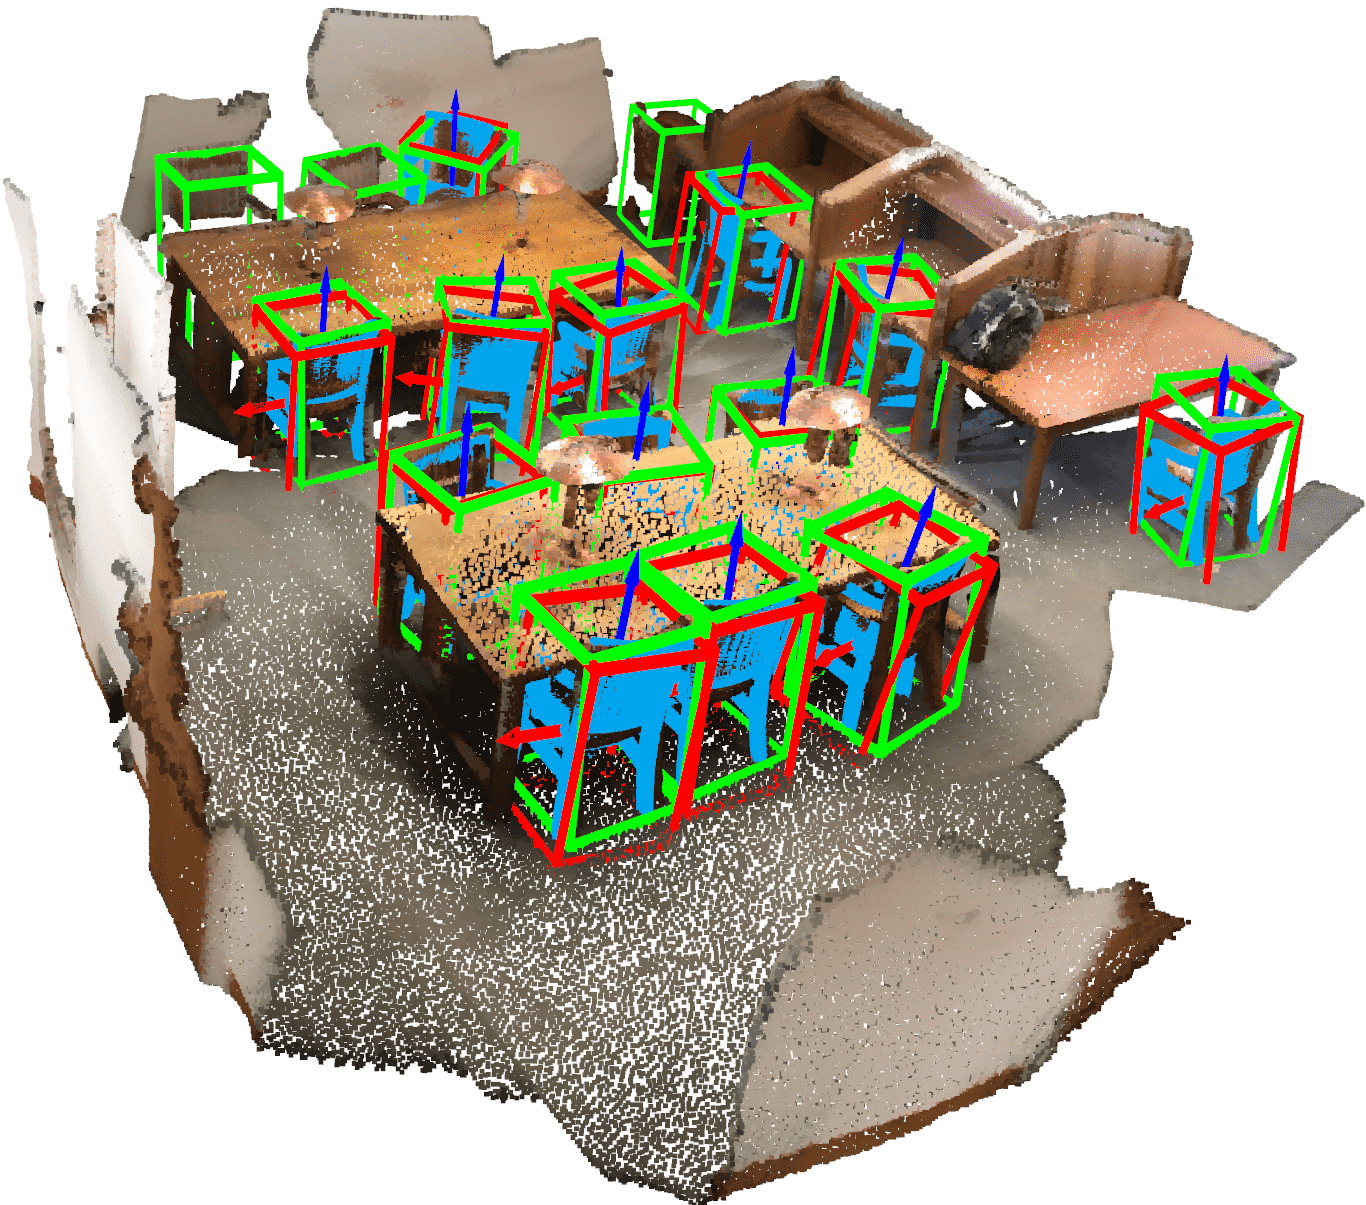
\includegraphics[height=2.8cm]{images/scan2cad-cad-ours1.png}
              \caption{Ours}
              \label{fig:scan2cad_cad-result1}
          \end{subfigure}
          \begin{subfigure}{0.18\textwidth}
            \centering
            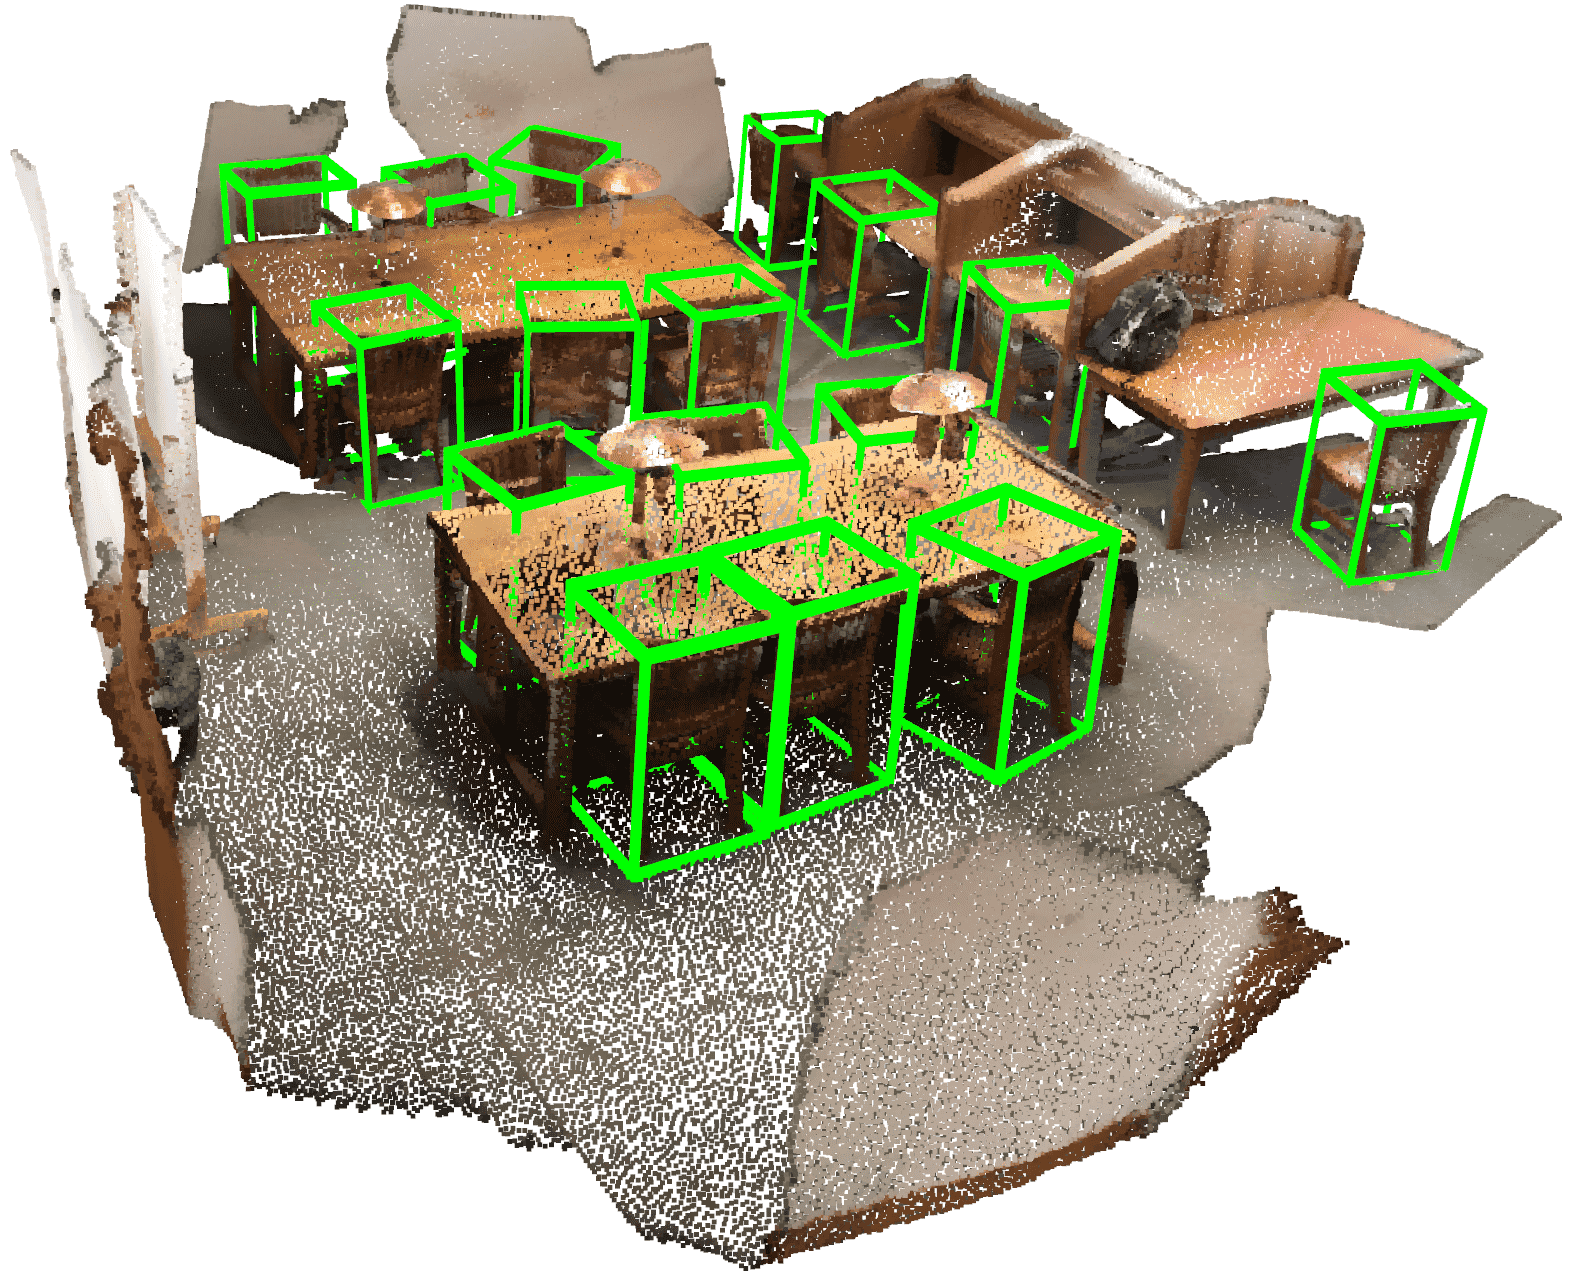
\includegraphics[height=2.8cm]{images/scan2cad-cad-tlinkage1.png}
              \caption{T-linkage\cite{magri2014t}}
              \label{fig:scan2cad_cad-tlinkage1}
          \end{subfigure}
          \begin{subfigure}{0.2\textwidth}
            \centering
            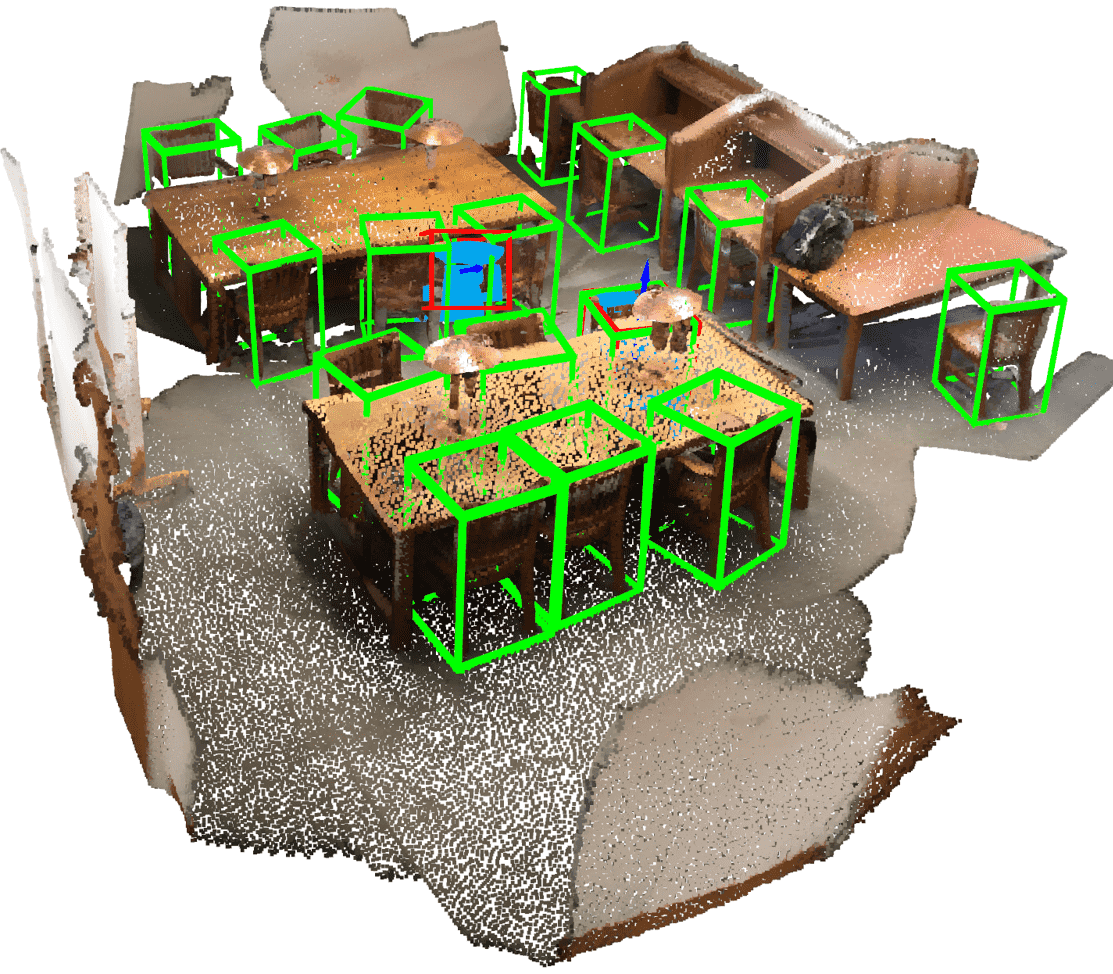
\includegraphics[height=2.8cm]{images/scan2cad-cad-progx1.png}
              \caption{Progressive-X\cite{zhao2021progressive}}
              \label{fig:scan2cad_cad-prox1}
          \end{subfigure}
          \begin{subfigure}{0.18\textwidth}
            \centering
            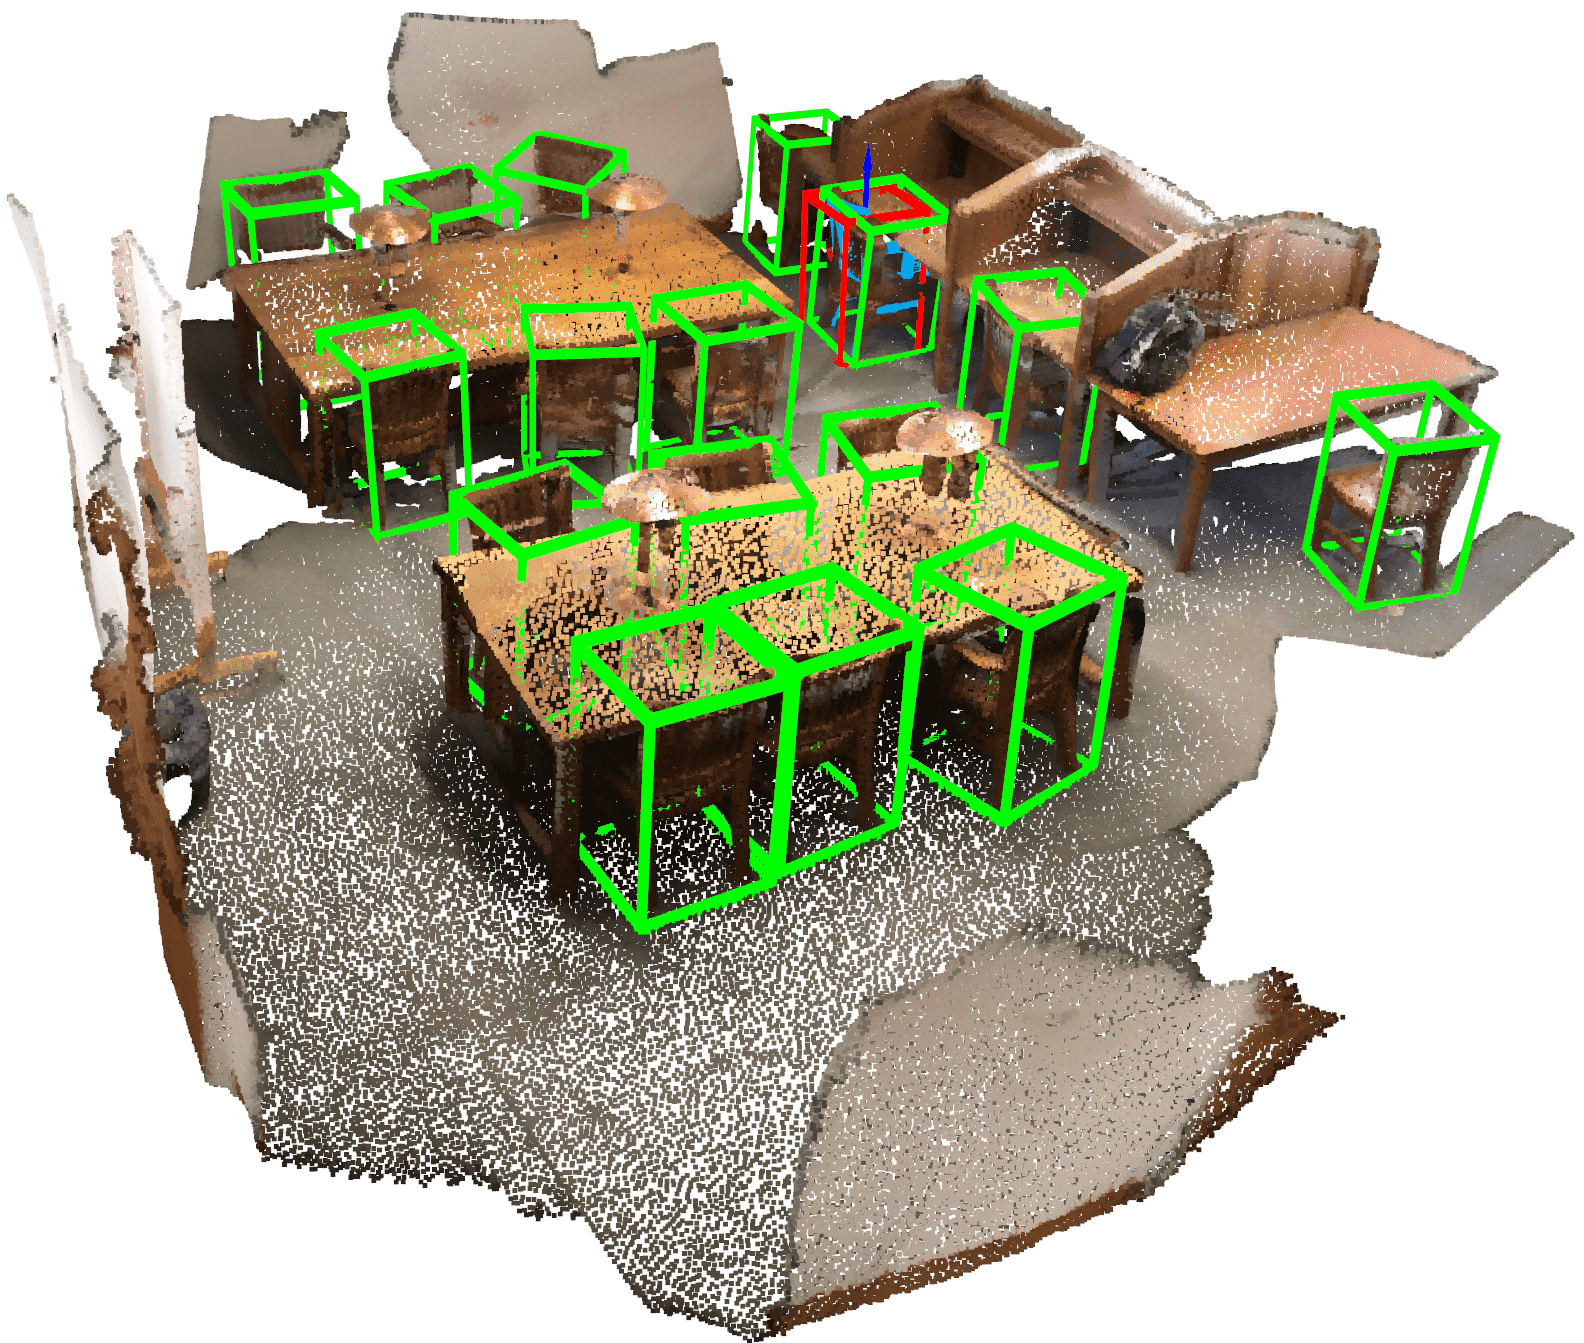
\includegraphics[height=2.8cm]{images/scan2cad-cad-consac1.png}
              \caption{CONSAC\cite{kluger2020consac}}
              \label{fig:scan2cad_cad-consac1}
          \end{subfigure}
          \begin{subfigure}{0.18\textwidth}
            \centering
            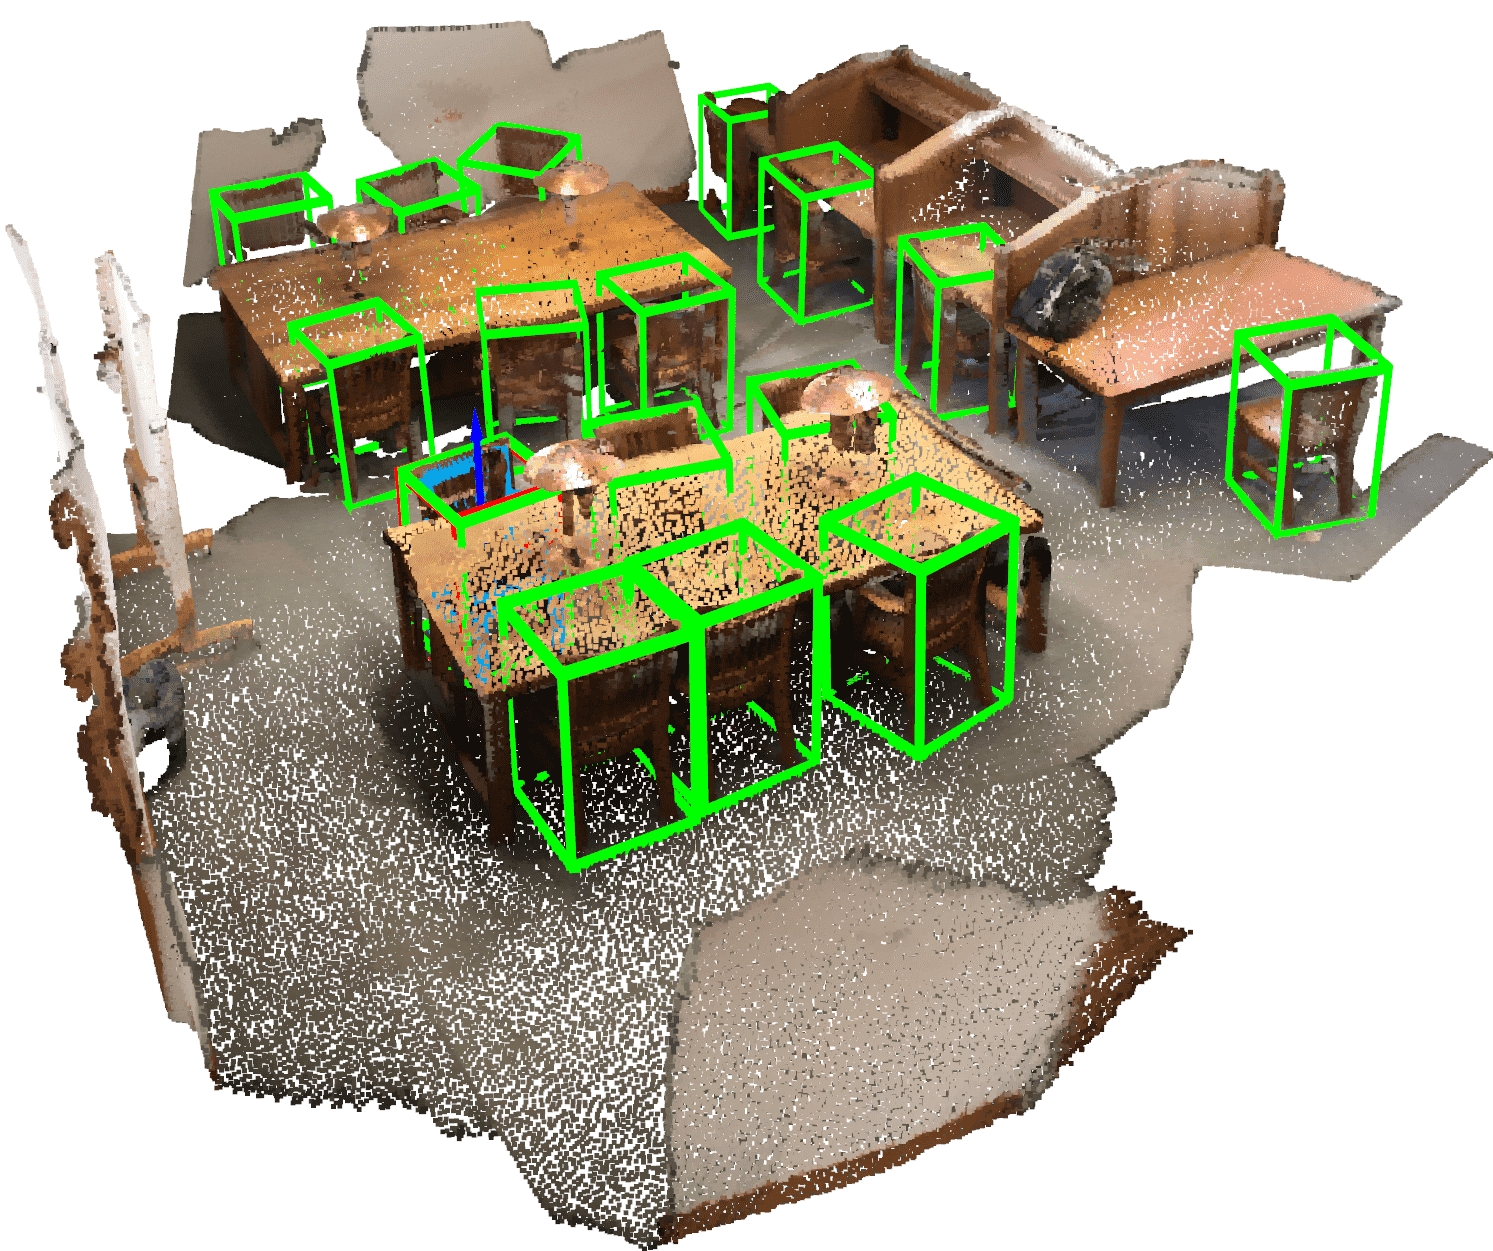
\includegraphics[height=2.8cm]{images/scan2cad-cad-teaser1.png}
              \caption{TEASER\cite{yang2020teaser}}
              \label{fig:scan2cad_cad-teaser1}
          \end{subfigure}
          % \begin{subfigure}{0.18\textwidth}
          %   \centering
          %   \includegraphics[height=2.5cm]{scan2cad-cad-ransac1.png}
          %     \caption{RANSAC}
          %     \label{fig:scan2cad_cad-ransac1}
          % \end{subfigure}
          \caption{\textbf{Scan2CAD 结果。} 我们的方法 (c) 在 16 个椅子中配准了 13 个实例。Progressive-X (e) 配准了 2 个实例,但其中一个的姿态误差较大。CONSAC (f) 和 TEASER (g) 都配准了一个实例。T-Linkage (d) 未能配准任何实例。}
    \label{fig:Scan2CAD-cadresult1}
    \end{figure*}
    

\begin{table}[h]
        \centering
        \resizebox{.75\columnwidth}{!}{
          \begin{tabular}{ccccc} %& $50\%~70\%$ & $70\%~90\%$
          \toprule
          \textbf{Metric}& MHR$\left( \% \right) \uparrow $& MHP$\left( \% \right) \uparrow $& MHF1$\left( \% \right) \uparrow $ & Time$\left( s \right) \downarrow $ \\
          \hline
          & \multicolumn{4}{c}{PREDATOR( estimated outlier ratio : $76.44\%$)} \\
          \hline
          T-Linkage & 2.46 & 3.79 & 2.71 & 1655.0 \\
          Progressive-X & 11.58 & 6.86 & 7.87 & 26.32\\
          CONSAC & 2.66 & 0.35 & 0.62 & 21.35\\
          \textbf{Ours} & \textbf{31.63} & \textbf{29.23} & \textbf{27.04} & \textbf{1.46/0.51} \\
          \hline
                          
          &\multicolumn{4}{c}{ D3Feat ( estimated outlier ratio :  $97.25\%$)} \\
          \hline
          T-Linkage & 0.04 & 0.22 & 0.06 & 2178.43 \\
          Progressive-X & \textbf{0.67} & \textbf{0.30} & \textbf{0.4} & 28.48 \\
          CONSAC & 0 & 0 & 0 & 21.88 \\
          \textbf{Ours} & 0.29 & 0.04 & 0.07 & \textbf{2.13/0.89} \\
        \bottomrule
        \end{tabular}
        }
          \caption{在Scan2CAD数据集上配准的结果。}
          \label{tab:Scan2CAD-cad}
\end{table}

\section{高效对应聚类的多实例点云配准}
\subsection{仿真数据集}
\subsubsection{仿真点对关系}
在这个测试中,我们直接通过混合真实值和离群值来生成输入对应关系。我们测试了不同的离群比例,$10\%\sim50\%$,$50\%\sim70\%$ 和 $70\%\sim90\%$。请注意,对于每个测试样本,离群点是在给定范围内随机抽样的。结果显示在表 \ref{tab:mm} 中。随着离群比例的增加,几乎所有方法的性能都有所下降,但我们的方法下降缓慢,且仍然明显优于其他方法。我们的算法在 CPU 或 GPU 上的速度比现有方法快 10 倍。
我们还在图 \ref{fig:detail-mm}(a) 中绘制了我们的方法在不同离群比例下的 MHF1(Mean Hit F1) 曲线,其中包括 $20$ 个实例。尽管当离群比例非常大时性能迅速下降,但我们的方法在 $70\%$ 的离群比例下仍然能达到 $90.46\%$ 的 MHF1。图 \ref{fig:detail-mm}(b) 显示了在固定离群比例 $50\%$ 的情况下,不同实例数量的 MHF1 曲线。即使存在 $30$ 个实例,我们的方法的 MHF1 也约为 $92.73\%$。

\begin{figure}[ht]
        \centering  
        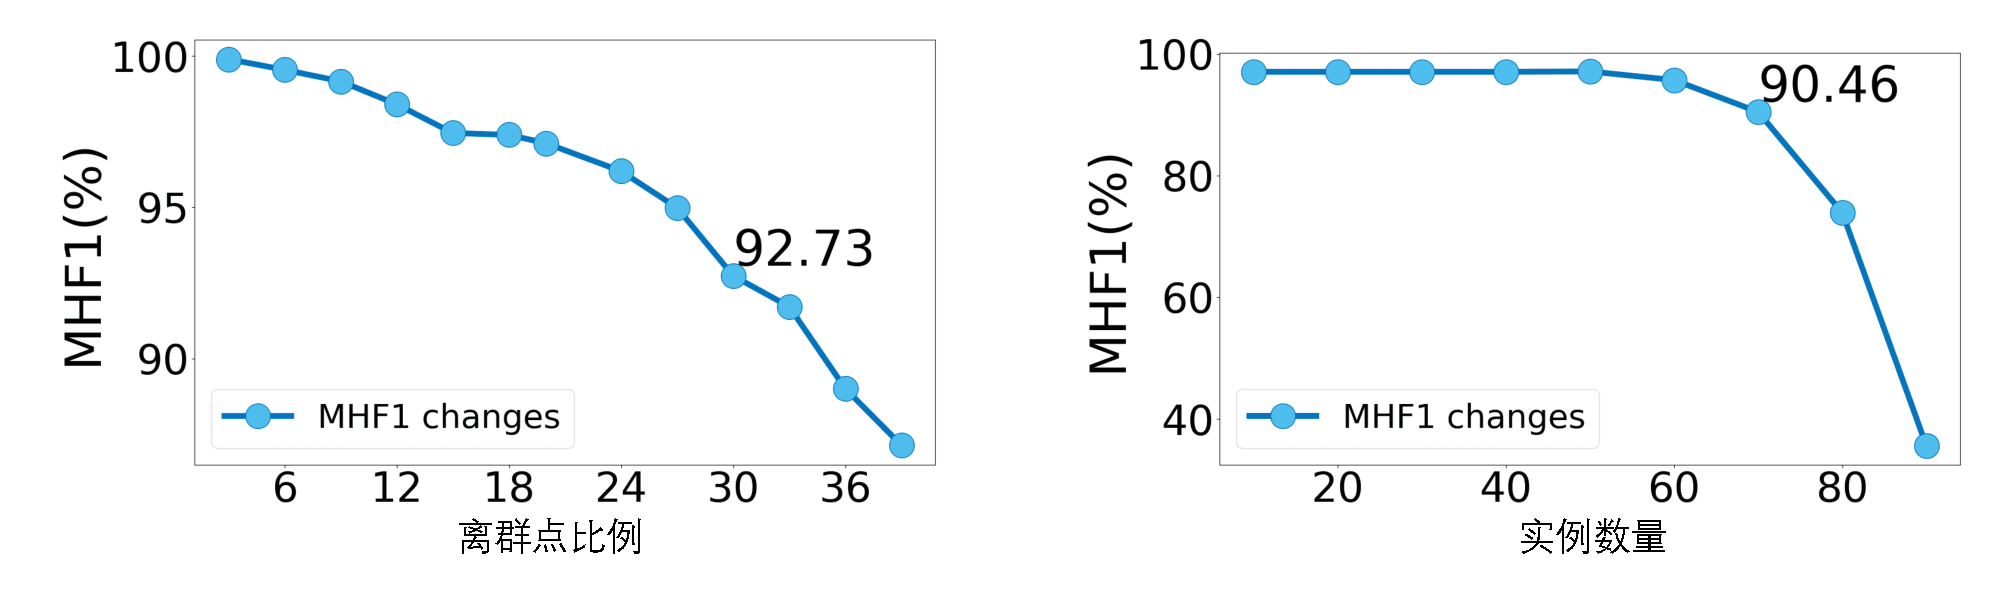
\includegraphics[width=\linewidth]{images/MHF1_curve.pdf}
        \caption{(a) 平均 Hit F1 与离群比例关系。 (b) 平均 Hit F1 与实例数量关系(固定离群比例为 $50\%$)。}
        \label{fig:detail-mm}
        %\label{fig:multi-instance}
\end{figure}

\subsubsection{基于特征的点对关系生成方式}

在此测试中,我们使用 PREDATOR\cite{huang2021predator} 和 D3Feat\cite{bai2020d3feat} 特征匹配来获得点对应关系。这两个特征模型都是在合成数据上训练的。结果显示在表 \ref{tab:realcorr} 中。值得注意的是,这两个特征都产生了超过 $90\%$ 的高离群点比例。在这样一个具有挑战性的情况下,我们的方法在鲁棒性和效率方面仍然表现良好,且明显优于现有方法。使用 D3Feat 的结果要比使用 PREDATOR 的结果差得多。原因不仅是因为更多的离群点,而且我们在检查结果时发现缺少内点。在后面的实验中我们在图 \ref{fig:predatormm} 中展示了一些结果。

\begin{table}[ht]
        \centering
        \resizebox{.75\columnwidth}{!}{
        \begin{tabular}{ccccc} %& $50\%~70\%$ & $70\%~90\%$
            \toprule
            % & MHR$\left( \% \right) \uparrow $ & MRRE $\left( \right) \downarrow $ & MRTE & Time\\
            \textbf{方法}& MHR$\left( \% \right) \uparrow $ & MHP$\left( \% \right) \uparrow $ & MHF1$\left( \% \right) \uparrow $ & 时间$\left( s \right) \downarrow $\\
            \hline
            \multicolumn{5}{c}{离群点比重 : $10\%\sim50\%$} \\
            \hline
            T-Linkage & 3.05 & 14.80 & 4.65& 57.27 \\
            Progressive-X & 27.91 & 80.28 & 41.04 & 87.25\\
            CONSAC & 0.47 & 0.47 & 0.47 & 9.23  \\
            \textbf{Ours} & \textbf{96.08} & \textbf{99.73} & \textbf{97.03} & \textbf{0.62/0.30} \\ % 前gt_num个预测值的recall
            \hline
            \multicolumn{5}{c}{离群点比重 : $50\%\sim70\%$} \\
            \hline
            %\hline
            % \textbf{metric} & MHR$\left( \% \right) \uparrow $ & RRE$\left( \degree \right) \downarrow $ & RTE$\left( m \right) \downarrow $ & t$\left( s \right) \downarrow $\\
            %\hline
            %\hline
            T-Linkage & 1.33 & 7.00 & 2.05 & 56.90 \\
            Progressive-X & 20.60 & 75.10 & 31.70 & 85.54  \\
            CONSAC & 0.49 & 0.49 & 0.49 & 9.55\\
            \textbf{Ours} & \textbf{93.99} & \textbf{99.49} & \textbf{95.51} & \textbf{0.55/0.28}\\
            \hline
            
            \multicolumn{5}{c}{Outlier ratio : $70\%\sim90\%$} \\
            \hline
            %\hline
            % \textbf{metric} & MHR$\left( \% \right) \uparrow $ & RRE$\left( \degree \right) \downarrow $ & RTE$\left( m \right) \downarrow $ & t$\left( s \right) \downarrow $\\
            %\hline
            %\hline
            T-Linkage & 0.81 & 4.42 & 1.25 & 56.89 \\
            Progressive-X & 12.88 & 62.60 & 20.73 & 84.5 \\
            CONSAC & 0.51 & 0.51 & 0.51 & 7.70  \\
            \textbf{Ours} & \textbf{60.39} & \textbf{94.42} & \textbf{69.36} &\textbf{0.50/0.24}\\
    
            \hline
            \multicolumn{5}{c}{离群点比重 : $90\%\sim99\%$} \\
            \hline
            T-Linkage & 0.28 & 1.30 & 0.42 & 56.69 \\
            Progressive-X & 7.13 & 39.19 & 11.67 & 84.43\\
            CONSAC & 0.51 & 0.51 & 0.51 & 9.57  \\
            \textbf{Ours} & \textbf{14.70} & \textbf{65.20} & \textbf{22.75} & \textbf{0.47/0.21} \\ % 前gt_num个预测值的recall
            \bottomrule
            %outlier ratio & $10\%~50\%$ & $50\%~70\%$ & $70\%~90\%$\\
    
        \end{tabular}
        }
        \caption{在不同离群比例的合成对应关系上的结果。$\uparrow$ 表示越大越好,而 $\downarrow$ 表示相反。我们方法在 CPU/GPU 上的运行时间也展示出来。}
        \label{tab:mm}
\end{table}

\begin{table}
        \centering
        \resizebox{0.75\textwidth}{!}{
            \begin{tabular}{ccccc} 
                \toprule
                \textbf{Metric}& MHR$\left( \% \right) \uparrow $& MHP$\left( \% \right) \uparrow $& MHF1$\left( \% \right) \uparrow $ & Time$\left( s \right) \downarrow $\\
                \hline
                & \multicolumn{4}{c}{PREDATOR ( estimated outlier ratio : $94.32\%$)} \\
                \hline
                T-Linkage & 0.19 & 0.54 & 0.27 & 43.46 \\
                Progressive-X & 15.90 & 31.01 & 18.98 & 86.39 \\
                CONSAC & 0.1 & 0.07 & 0.08 & 7.65 \\
                \textbf{Ours} &\textbf{53.39} & \textbf{61.44} & \textbf{51.80} & \textbf{1.28/0.48} \\
                \hline
                
                &\multicolumn{4}{c}{D3Feat ( estimated outlier ratio : $99.30\%$)} \\
                \hline
                %\hline
                % \textbf{metric} & MHR$\left( \% \right) \uparrow $ & RRE$\left( \degree \right) \downarrow $ & RTE$\left( m \right) \downarrow $ & t$\left( s \right) \downarrow $\\
                %\hline
                %\hline
                T-Linkage & 0.07 & 0.29 & 0.1 & 56.37  \\
                Progressive-X & 4.29 & 15.28 & 5.94 & 87.22 \\
                CONSAC & 0.13 & 0.04 & 0.05 & 9.53 \\
                \textbf{Ours} & \textbf{16.98} & \textbf{27.05} & \textbf{17.91} & \textbf{0.68/0.30} \\
                \bottomrule
        \end{tabular}
        }
        \caption{使用特征匹配在合成数据上生成对应点的结果。部分结果可在图 \ref{fig:predatormm} 中进行可视化。}
        % \caption{Results on synthetic data using feature matching to generate correspondences.$\uparrow$ means the larger the better, while $\downarrow$ indicates the contrary. The running time on CPU/GPU of our method is presented. Some results are visualized in Figure \ref{fig:predatormm}.}
        \label{tab:realcorr}
\end{table}

\subsection{真实数据集}
在真实数据集中的测试结果如表 \ref{tab:Scan2CAD-cad} 所示。我们的方法在使用 PREDATOR 时明显优于现有方法。请注意,当使用 D3Feat 时,所有方法的性能都很差。在仔细检查结果后,我们发现原因不仅是高异常值比率(约 $97.25\%$),而且在使用 D3Feat 时,即使特征匹配仅限于目标点云中的真实边界框内,内点也不足。一些结果如图 \ref{fig:Scan2CAD-cadresult} 和图 \ref{fig:Scan2CAD-cadresult1} 所示。


\section{基于深度学习的多实例点云配准}
\subsection{仿真数据集}
我们首先将基于深度学习的方法与仿真数据集上的其他竞争者进行比较,结果如表 \ref{table1} 所示。
由于内点比例极低,基于采样的方法如 T-Linkage、RansaCov 和 CONSAC 的性能不佳。
由于空间一致性的优势,ECC 表现出有效性。
然而,我们的 DMR 在所有评价指标上均大幅度超越了第二好的方法 ECC。

\setlength{\tabcolsep}{8pt}
\begin{table}[ht]
  \centering
  \caption{在合成数据集上的配准结果。}
  \begin{tabular}{ccccc}
    \hline\noalign{\smallskip}
  & MR(\%)         & MP(\%)         & MF(\%)         & Time(s)       \\
  \noalign{\smallskip}
  \hline
  \noalign{\smallskip}
  T-linkage \cite{magri2014t} & 0.61           & 1.48           & 0.87           & 3.89          \\
  RansaCov \cite{magri2016multiple}  & 0.73           & 5.33           & 1.29           & 0.14          \\
  CONSAC \cite{kluger2020consac}    & 1.00           & 7.45           & 1.77           & 0.61          \\
  ECC         & 82.90          & 92.92          & 87.63          & 3.56          \\
  DMR              & \textbf{92.60} & \textbf{99.69} & \textbf{96.01} & \textbf{0.06} \\
  \hline
  \end{tabular}
  \label{table1}
\end{table}

为了定性评估我们的PointCLM并将其与其他竞争者进行比较,我们在图\ref{fig:DMR}中提供了一组可视化。图\ref{fig:DMR}的第一行显示了输入对应关系,以及我们的剪枝和聚类结果。图\ref{fig:DMR}(b)显示,我们的PointCLM惊人地去除了所有的离群点,剩余的对应关系在图\ref{fig:DMR}(c)中被很好地聚类。

图\ref{fig:DMR}的第二行显示了我们提出的方法和竞争者的配准结果。可以看到,T-Linkage和RansaCov都无法配准任何实例。对于目标点云中的六个实例,CONSAC只成功配准了一个实例。值得注意的是,尽管ECC成功配准了四个实例,但它未能配准右下角的两张桌子。这是因为这两张桌子混在一起,空间一致性不足以区分它们。然而,我们的方法成功配准了所有实例。

\begin{figure}
        \centering
        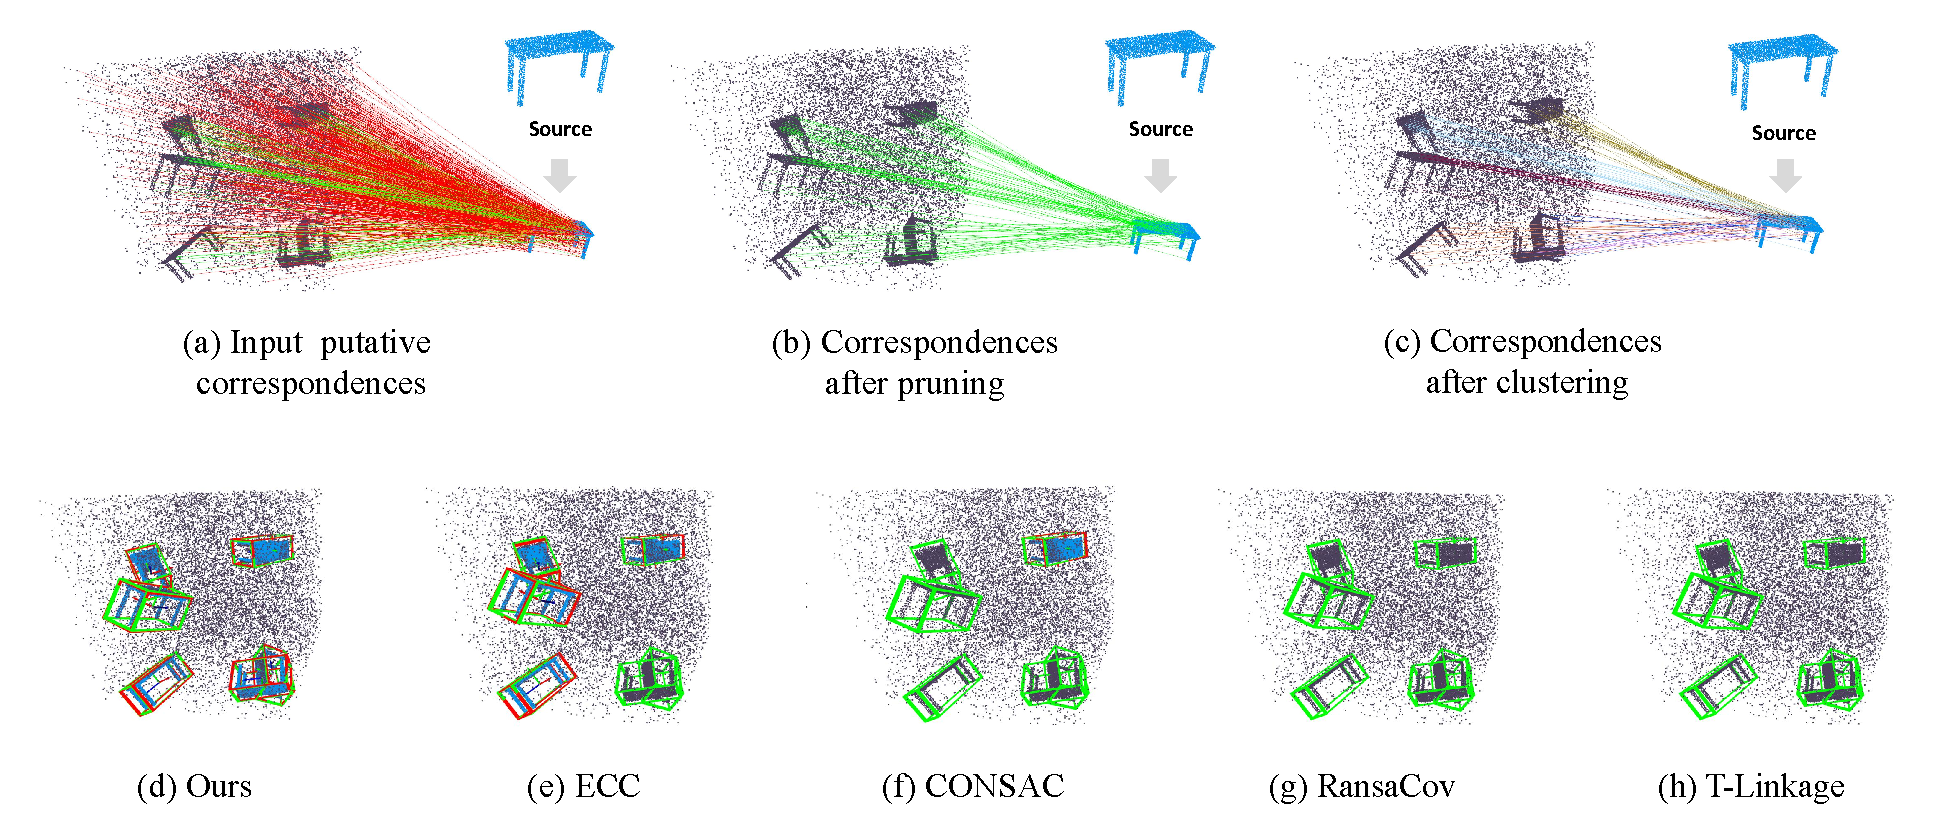
\includegraphics[width=1.0\textwidth]{images/DMR_syn.pdf}
        \caption{
                在合成数据集上的结果。
                在(a)和(b)中,绿线和红线分别代表内点对应关系和异常值对应关系。
                在(c)中,聚类后每个簇中的对应关系以不同的颜色可视化。
                在(d-f)中,绿色边界框表示目标点云中实例的真实姿态,红色边界框表示预测。
                目标点云中的变换点云以蓝色可视化。
        }
        \label{fig:DMR}
\end{figure}

\subsection{真实数据集}
\begin{table}[ht]
        \centering
        \caption{配准结果在真实数据集上.}
        \begin{tabular}{ccccc}
        \hline\noalign{\smallskip}
        & MR(\%)         & MP(\%)         & MF(\%)         & Time(s)       \\
        \noalign{\smallskip}
        \hline
        \noalign{\smallskip}
        T-linkage  & 34.99          & 46.86          & 40.07          & 6.64          \\
        RansaCov   & 60.50          & 33.28          & 42.94          & \textbf{0.07} \\
        CONSAC     & 55.48          & 53.34          & 54.39          & 0.39          \\
        ECC        & 64.66          & 69.73          & 67.10          & 1.84          \\
        DMR   & \textbf{78.10} & \textbf{70.64} & \textbf{74.18} & 0.10        \\ 
        \hline
        \end{tabular}
        \label{tab:DMR_real}
\end{table}
      
如表 \ref{tab:DMR_real}所示,我们的PointCLM在所有三个评估指标,MR,MP和MF上均优于所有竞争者,速度也很有竞争力。 
ECC和PointCLM的性能低于合成数据集,而其他方法的性能高于合成数据集。 
这是由于实例内点比率分布的变化。 
      
我们还提供了一组可视化,以定性评估我们的PointCLM并与其他竞争者进行比较。 
图 \ref{fig:DMR_real}的第一行显示了输入对应关系,以及我们的剪枝和聚类结果。 
图 \ref{fig:DMR_real}(b)表明,我们的方法几乎去除了所有的异常值,确保了如图 \ref{fig:DMR_real}(c)所示的后续聚类高效执行。 
对于包含在目标点云中的五个实例,T-Linkage和CONSAC成功配准了两个实例,但T-Linkage的一个预测有大的错误。 
RansaCov成功配准了三个实例。 
由于目标点云中的三把椅子靠得很近,ECC并没有成功配准所有这些实例。 
我们的方法成功完成了所有实例的配准。
      
\begin{figure}
        \centering
        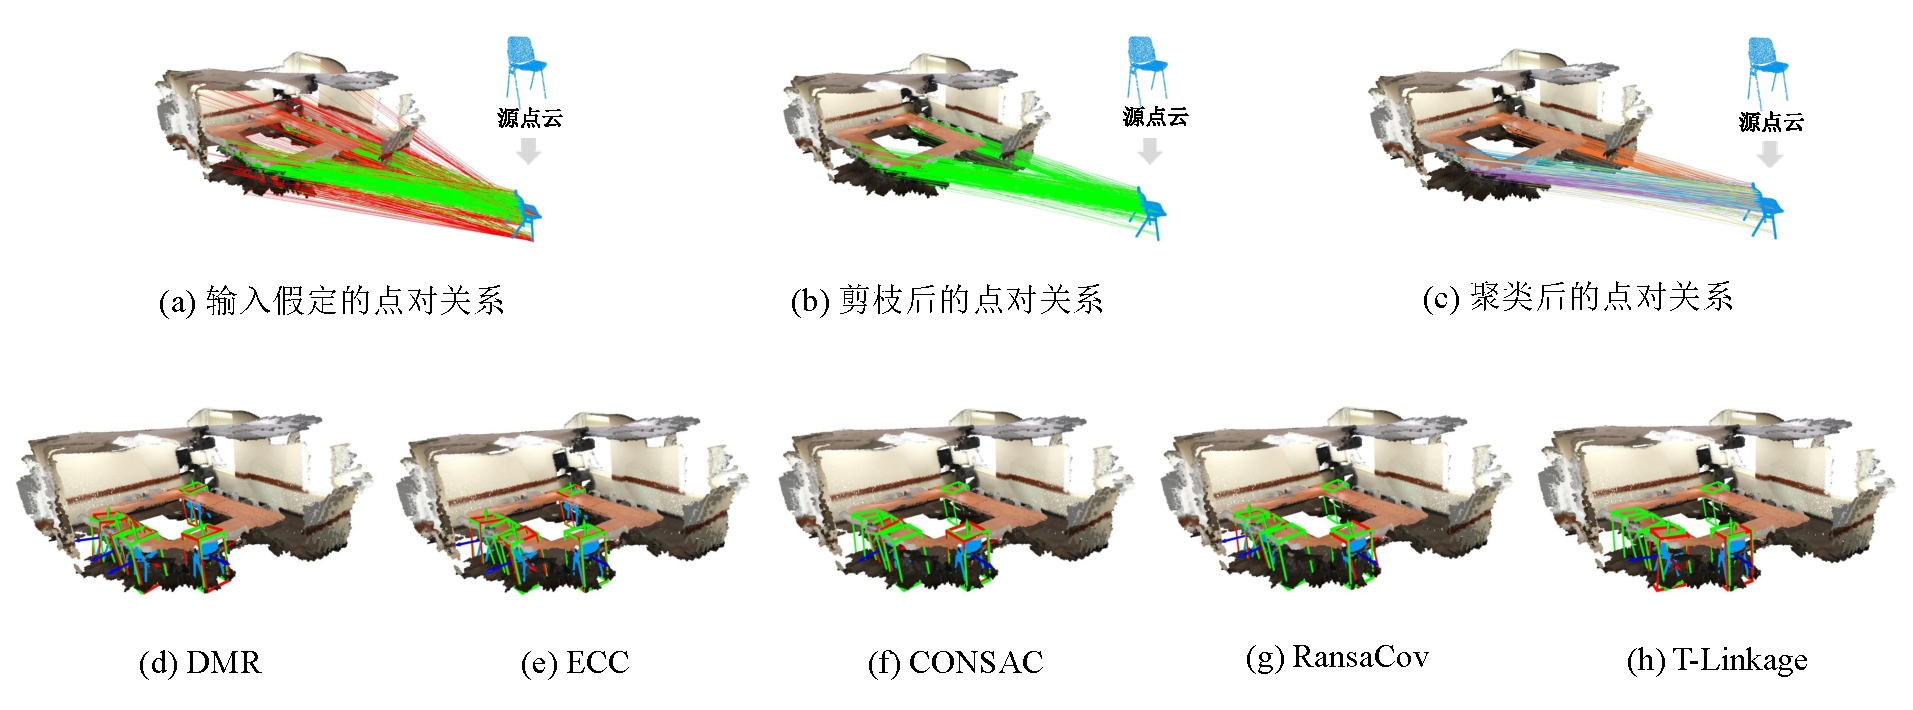
\includegraphics[width=1.0\textwidth]{images/DMR_real.pdf}
        \caption{
          在真实数据集上的结果。
          在(a)和(b)中,绿线和红线分别代表内点对应关系和异常值对应关系。
          在(c)中,聚类后每个簇中的对应关系以不同的颜色可视化。
          在(d-f)中,绿色边界框表示目标点云中实例的真实姿态,红色边界框表示预测。
          目标点云中的变换点云以蓝色可视化。
        }
        \label{fig:DMR_real}
\end{figure}
      
\subsection{消融实验}
\label{sec:ablation}
\subsubsection{深度表示的消融研究}为了研究我们采用的深度表示的有效性,我们比较了我们的框架在有和无深度表示下的性能。
没有深度表示的版本删除了特征提取器并设置 $S=\beta$,只依赖空间一致性进行剪枝和聚类。
比较结果如表 \ref{tab:ablation} 所示。
可以看到,使用深度表示后,准确性和速度指标都有所提高。
没有深度表示,剪枝的对应关系少,需要聚类的对应关系多,这增加了我们方法的运行时间。
尽管没有深度表示的框架在MR、MP和MF上的性能较低,但它仍然是一个有竞争力的基线,适合没有训练数据的情况。
这表明了本文提出的剪枝和聚类策略的有效性。

此外,我们在图 \ref{fig:spectral} 中可视化了有无深度表示的聚类结果。
我们选择了一个例子,其目标点云包含三个实例。
我们首先使用一个3维的one-hot向量来表示一个对应关系属于哪个实例。
然后我们使用这些向量来计算相似性矩阵,并使用聚类的结果对这些矩阵进行排列。
可以看到,通过深度表示排列的相似性矩阵比没有深度表示的框架排列的相似性矩阵小得多,因为在前者的情况下,剪枝过程中去除了更多的异常值。
更重要的是,图 \ref{fig:spectral}(b) 中的矩阵显示了三个明显的簇,这些簇对应于三个实例。
相反,图 \ref{fig:spectral}(a) 中的矩阵显示了两个块,其中右下角的块实际上对应于两个实例,如果不使用提出的深度表示,无法成功区分。

\setlength{\tabcolsep}{2pt}
\begin{table}
  \caption{
    深度表示和剪枝的消融研究结果。
    }
  \centering
  \begin{tabular}{cccccc}
    \hline\noalign{\smallskip}
    深度表示 & 剪枝 & MR(\%)         & MP(\%)         & MF(\%)         & Time(s)       \\
  \noalign{\smallskip}
  \hline
  \noalign{\smallskip}
  & $\checkmark$       & 76.61          & 65.05          & 70.36          & 0.17          \\
  $\checkmark$                   &         & 62.23          & 32.77          & 42.93          & 1.24          \\
  $\checkmark$                &
 $\checkmark$     & \textbf{78.10} & \textbf{70.64} & \textbf{74.18} & \textbf{0.10}\\
  \hline
  \end{tabular}
  \label{tab:ablation}
\end{table}
\setlength{\tabcolsep}{1.4pt}


\begin{figure}
  \centering
  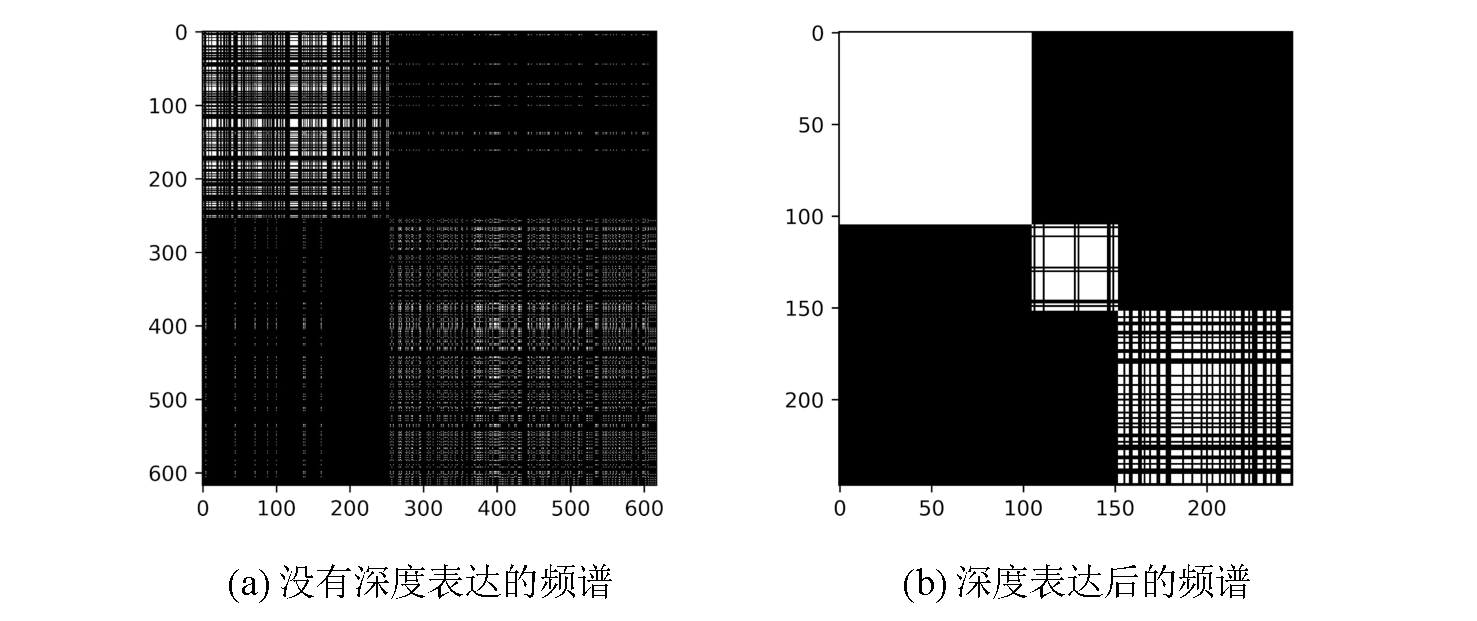
\includegraphics[width=0.8\textwidth]{images/spectral.pdf}
  \caption{
    无深度表示和有深度表示的聚类结果可视化。
    }
  \label{fig:spectral}
\end{figure}

\subsubsection{对修剪的消融研究}为了定量研究我们的修剪策略的有效性,我们简单地在我们的方法中去除修剪策略,然后比较去除前后的性能。
表 \ref{tab:ablation} 显示,如果去除修剪步骤,我们的方法的性能会大幅下降,这是由于噪声二进制相似性矩阵不符合 \cite{li2007noise} 定义的理想矩阵,光谱聚类无法正确地对应关系进行分组。
这个结果表明,修剪对后续的聚类至关重要。

\subsubsection{对 RANSAC 迭代次数的消融研究}此外,我们还测试了我们的模型在不同的 RANSAC 迭代次数下的性能,结果如表 \ref{tab:ransac} 所示。
可以看到,只用五次迭代就可以得到相当好的结果,而 50 次和 500 次迭代的性能非常接近。
这些结果表明,修剪和聚类步骤极大地提高了每个实例的内点比例,因此,只使用少量的迭代次数就可以估计出可靠的结果。


\begin{table}
  \caption{
        RANSAC 迭代次数的影响
  }
  \centering
  \begin{tabular}{cccc}
    \hline\noalign{\smallskip}
    RANSAC 次数 & MR(\%)         & MP(\%)         & MF(\%)          \\
  \noalign{\smallskip}
  \hline
  \noalign{\smallskip}
  5   & 77.39          & 67.76          & 72.26              \\
  50  & 78.10          & \textbf{70.64} & 74.18                \\
  500 & \textbf{79.33} & \textbf{70.64} & \textbf{74.73}  \\  
  \hline
  \end{tabular}
  \label{tab:ransac}
\end{table}

\subsubsection{关于最难负样本消融研究}
为每个小批量找到最困难的负对会产生更大的计算开销,但我们的消融研究显示这是值得的。
我们将其与使用随机选择的负对训练的相同模型进行比较。
使用最困难的负对(如本方法所述)和使用随机选择的负对的结果如表 \ref{tab:hardest} 所示。
所有的准确性指标都通过在对比学习中使用最困难的负对得到了提升。
通过比较表 \ref{tab:hardest} 和表 \ref{tab:ablation},我们可以发现,在对比表示学习中使用随机负对得到的结果优于不使用深度表示,但差距很小。
此外,我们在表 \ref{tab:hardest} 中收集了特征空间中正对和 top-K 最困难的负对的平均余弦相似性。
结果显示,使用最困难的负对训练的表示在特征空间中更好地分离,更具区分性。

\begin{table}
  \caption{
        用最难的负样本进行训练的消融实验结果。
  }
  \centering
  \begin{tabular}{ccccccc}
    \hline\noalign{\smallskip}
    & MR(\%) & MP(\%) & MF(\%) & Positive(\%) & Top-1(\%) & Top-10(\%) \\
    \noalign{\smallskip}
    \hline
    \noalign{\smallskip}
    随机  & 76.85  & 67.50  & 71.87  & 95.43 & 96.91 & 91.37  \\
    最难 & \textbf{78.10} & \textbf{70.64} & \textbf{74.18} & 83.96 & 61.32 & 49.65 \\  
    \hline
  \end{tabular}
  \label{tab:hardest}
\end{table}


\section{小结}
本章,我们对提出的两种多实例点云配准模型进行了广泛的实验评估,包括定量的实验评估和可视化的实验评估,并且对基于深度学习的方法进行了广泛的消融实验。其中基于深度学习的方法效果超过了单纯的聚类算法,证明了深度学习方法在多实例点云配准中的有效性,学习鲁棒的点对特征能够大大增大配准的效果。